\documentclass[twocolumn]{aa}
\usepackage{graphicx}
\usepackage{multirow}
\usepackage{enumitem} % for no indent in itemize 
\usepackage[]{algorithm2e}
\newcommand{\vdag}{(v)^\dagger}
%\newcommand\aastex{AAS\TeX}
\newcommand\latex{La\TeX}
\usepackage{xcolor}
\usepackage{subfigure}
\usepackage[normalem]{ulem}
\usepackage{mathtools}
\usepackage{amsmath}
\usepackage[colorlinks=true, allcolors=blue]{hyperref}
%\newcommand{\mathcolorbox}[2]{\colorbox{#1}{$\displaystyle #2$}}
%\newcommand{\hlfancy}[2]{\sethlcolor{#1}\hl{#2}}

\usepackage{txfonts}
\usepackage{textcomp} % for \textmu

\usepackage{ulem}
\newcommand{\anthony}[1]{\textcolor{magenta}{#1}} 
\newcommand{\olivier}[1]{\textcolor{orange}{#1}}
\newcommand{\og}[2]{\textcolor{orange}{\sout{#1} {#2}}}
\newcommand{\tc}[1]{\textcolor{green}{#1}} %Thayne's corrections
\newcommand{\nour}[1]{\textcolor{teal}{#1}}
\renewcommand{\v}[1]{\textcolor{red!70!white}{#1}}
\newcommand{\vs}[1]{\textcolor{red!70!white}{\sout{#1}}}

% Main

\begin{document}


   \title{On-sky validation of image-based adaptive optics wavefront sensor referencing}

   %\subtitle{I. Overviewing the $\kappa$-mechanism}


%\title{Do you trust your reference?}
%On-sky correction of static and quasi-static non-common path aberration with the pyramid wavefront sensor in Extreme Adaptive Optics.
%DrWHO 1.0: Non-common path aberrations with the pyramid wavefront sensor: how much do you actually trust your reference?
%\correspondingauthor{Nour Skaf}

\author{Nour Skaf\inst{\ref{inst:LESIA},\ref{inst:Subaru},\ref{inst:UCL}} \and%
    %Olivier Guyon\inst{\ref{inst:Subaru},\ref{inst:ABC},\ref{inst:UoA}, \ref{inst:UoAO}}
	%Éric Gendron\inst{\ref{inst:LESIA}} \and%
	%Anthony Boccaletti\inst{\ref{inst:LESIA}} \and%
	%Arielle Bertrou-Cantou\inst{\ref{inst:LESIA}} \and%
	%Kyohoon Ahn\inst{\ref{inst:Subaru}} \and%
	%Jesse Cranney\inst{\ref{inst:ANU}} \and%
	%Thayne Currie\inst{\ref{inst:Subaru},\ref{inst:Ames}}\and%
	%Vincent Deo\inst{\ref{inst:Subaru}} \and%
	%Billy Edwards\inst{\ref{inst:UCL}} \and%
	%Florian Ferreira\inst{\ref{inst:LESIA}} \and%
	%Damien Gratadour\inst{\ref{inst:LESIA},\ref{inst:ANU}}\and\\%
	%Julien Lozi\inst{\ref{inst:Subaru}}\and%
	%Barnaby Norris\inst{\ref{inst:SydneyUni}} \and 
	%Arnaud Sevin\inst{\ref{inst:LESIA}} \and%
	%Fabrice Vidal\inst{\ref{inst:LESIA}} \and%
	%Sébastien Vievard\inst{\ref{inst:Subaru},\ref{inst:ABC}}
	}%
	
\institute{LESIA, Observatoire de Paris, Univ.~PSL, CNRS, Sorbonne Univ., Univ.~de Paris, 5 pl. Jules Janssen, 92195 Meudon, France\label{inst:LESIA}%
\and %
National Astronomical Observatory of Japan, Subaru Telescope, 650 North A'oh\=ok\=u Place, Hilo, HI 96720, U.S.A.\label{inst:Subaru} %
\and 
Department of Physics and Astronomy, University College London, London, United Kingdom\label{inst:UCL} %
\and 
%Astrobiology Center of NINS, 2-21-1 Osawa, Mitaka, Tokyo 181-8588, Japan\label{inst:ABC}
\and
%Steward Observatory, University of Arizona, Tucson, AZ 85721, USA\label{inst:UoA}
\and
%College of Optical Sciences, University of Arizona, Tucson, AZ 85721, USA\label{inst:UoAO}
\and %
%Research School of Astronomy and Astrophysics, Australian National University, Canberra, ACT 2611, Australia\label{inst:ANU} %
%\and
%NASA-Ames Research Center, Moffett Field, California, USA\label{inst:Ames}
%\and
%Sydney Institute for Astronomy, School of Physics, University of Sydney, NSW 2006\label{inst:SydneyUni}
\\
email: \texttt{nour.skaf@obspm.fr}
}

 
   \date{Received XXX; accepted XXX}

%\begin{abstract}

%below is the first astract draft 
{
%Exoplanetary science is a rapidly growing field in astronomy. However, detecting an exoplanet is very challenging. Over the last couple of decades, ground-based and space-based telescopes became more and more focused on this purpose, using a variety of detection techniques, with the goal to eventually find a nearby planet in the habitable zone with the next generation of instruments. The technique of direct imaging will play a key role in this search. Our project will directly address this challenge of direct detection and characterisation of exoplanets, by developing and testing high precision adaptive optics control techniques to compensate for atmospheric optical turbulence, and the non-common paths aberrations (NCPAs). The problem of NCPAs is key in direct imaging, as it is one of the main sources of residual speckles in the PSF. The  pyramid  wavefront  sensor  (PyWFS),  more  and  more  favored  in  adaptive optics systems for its high sensitivity, is intimately linked with the NCPAs correction.  However, the PyWFS is non-linear, making its use more challenging.  We will leverage newly available real-time computing capabilities and machine learning numerical tools in order to tackle those problems of NCPAs corrections with a PyWFS, for boosting image contrast and quality to reveal planet images and better characterise them. We will present the DrWHO algorithm, which is kind of reinforcement learning approach for frequency lucky imaging and update on-sky the PyWFS reference.\\



% below is the submitted for WFS in the VLT era. \\
%Exoplanetary science is a rapidly growing field in astronomy. However, detecting directly an exoplanet is very challenging. Over the last couple of decades, ground-based telescopes became more and more focused on this purpose, using a variety of wavefront control techniques. The proposed method directly addresses this challenge, by developing and testing high precision adaptive optics control techniques to compensate for optical aberrations other than the atmospheric ones, the non-common paths aberrations (NCPAs). The problem of NCPAs is key in direct imaging, as it is one of the main sources of residual speckles in the stellar field.
%We present DrWHO - Direct Reinforcement Wavefront Heuristic Optimisation -, an algorithm aimed at quasi-real-time compensation of NCPAs, for boosting image contrast and quality to reveal planet images and better characterize them. It is a kind of reinforcement learning approach for frequency lucky imaging and update on-sky the pyramid wavefront sensor (PyWFS) reference.
%We show that DrWHO does not require accurate wavefront sensor calibration, and is applicable to non-linear wavefront sensing situations. We demonstrate its performance in simulation and on-sky using with the PyWFS sensor.

%\end{abstract}

%\keywords{Astronomy instrumentation, Adaptive Optics, Extreme Adaptive Optics}
}


  \abstract
  % context heading (optional)
  % {} leave it empty if necessary
   {
   %\v{What about including RL in the title? "Reinforcement learning for non-linear wavefront sensor self-referencing" or the like ?} 
   Differentiating between a true exoplanet signal and residual speckle noise is a key challenge in high-contrast imaging (HCI).
   %A key challenge in high contrast imaging (HCI) is to differentiate an exoplanet signal from speckle noise. 
   Speckles are due to a combination of fast, slow and static wavefront aberrations introduced by atmospheric turbulence and instrument optics.
   While wavefront control techniques developed over the last decade have shown promise in minimizing fast atmospheric residuals, slow and static aberrations like non-common path aberrations (NCPAs) remain a key limiting factor for exoplanet detection.
   %Over the last decade, wavefront control techniques have been developed to minimize fast atmospheric residuals, such that slow and static aberrations, such as non-common path aberrations (NCPAs), are now the limiting factor in detection limits. 
   NCPAS are not seen by the wavefront sensor (WFS) of the adaptive optics (AO) loop, hence the difficulty in correcting them.}
   %and require open-loop offsetting, a challenge with non-linear WFSs.}}
  % aims heading (mandatory)
   {
   %Our method directly addresses the challenge of identifying and compensating slow and static aberrations, generating residual speckles in adaptive optics-corrected images. 
   We propose to improve the identification and rejection of slow and static speckles in AO-corrected images.
   The algorithm DrWHO - Direct Reinforcement Wavefront Heuristic Optimisation -, performs frequent compensation of static and quasi-static  
   %\anthony{(what is the point of real time for static aberrations? we should probably focus on the quasi-static term. instead of "real time" can we say "frequent")} 
   aberrations (including NCPAs) to boost image contrast and quality for general purpose AO systems as well as HCI systems. 
   %\anthony{already mentioned above, so not necessary:}
   %Residuals speckles are especially critical for exoplanet imaging, as they mimic an exoplanet signal 
   %to reveal planet images and better characterize them.
   }
  % methods heading (mandatory)
   {By changing the WFS reference at every iteration of the algorithm (few tens of seconds), DrWHO changes the AO system point of convergence to lead it towards a compensation of the static and slow aberrations. 
   %It does so by changing the WFS reference at every iteration of the DrWHO loop.
   References are calculated using an iterative lucky-imaging approach, where each iteration updates the WFS reference, ultimately favoring high-quality focal plane images. 
   %
   }
  % results heading (mandatory)
   {We validate this concept through both numerical simulations and on-sky %on 
   testing on the SCExAO instrument at the 8-m Subaru telescope. Simulations show a rapid convergence towards the correction of 82\% of the NCPAs. On-sky tests were perform over a 10-minute run in the visible (750~nm). We introduce a flux concentration (FC) metric to quantify the point spread function (PSF) quality and measure a  12\% improvement compared to the pre-DrWHO image.}
  % conclusions heading (optional), leave it empty if necessary
   {The DrWHO algorithm is a robust focal-plane wavefront sensing calibration method that has been successfully demonstrated on sky. It does not rely on a model and does not require wavefront sensor calibration or linearity. It is compatible with different 
   %\anthony{(other than what? you did not introduce the WFC method of scexao)} 
   wavefront control methods, and can be further optimized for speed and efficiency. 
   The algorithm is ready to be incorporated in scientific observations, enabling better PSF quality and stability during observations.}

   \keywords{Astronomical instrumentation, methods and techniques, Adaptive Optics, Numerical}

   \maketitle



\section{Introduction} \label{sec:intro}
%T.C - this needs some rephrasing
Over the past 30 years, Adaptive Optics (AO) instrumentation has undergone extensive growth in sophistication and scientific capabilities. Compared to the first astronomical AO experiments with the COME-ON system consisting of a 19-actuator deformable mirror (DM) driven at several hundred Hz \citep{Kern1989,Rousset1990}, current leading extreme AO (xAO) systems consists of 2000-actuator DMs driven at over 1 kHz speeds \citep[e.g.][]{GPIMacintosh2014,Beuzit2019}. The high-contrast imaging enabled by these new AO capabilities has led to key scientific breakthroughs, including the first direct image of a planet-mass companion \citep{chauvin2004} and the first imaged system of jovian exoplanets \citep{Marois2008}.  
%\citep{Mill2016
%Over the last 30 years, adaptive optics (AO) instruments have seen a tremendous progress in terms of development and scientific use, from the first experiments in astronomy with COME-ON, back in 1989, to the most current advanced systems known as extreme AO (xAO) systems. Many scientific breakthrough came from AO instruments, including the first detection of a planetary companion with VLT/NaCo in 2004 \citep{chauvin2004}, and the first system with four giant planets, HR8799, discovered in 2008 \citep{Marois2008}. In the following years, a second generation of xAO systems was developed, allowing to go much further in performance in terms of Strehl ratio, contrast, and sensitivity. \cite{Milli2016} made a comparison between AO and xAO systems, in the context of high contrast imaging of exoplanets. 

%\olivier{(This section makes claims about SCExAO and MAgAO-X being superior to SPHERE and GPI that are too broad and not exact. For example, SPHERE and GPI are probably more stable. Lets remove these comparisons and just mention that SCExAO and MagAO-X are exploring newer WFS/C approaches with a focus to serve as prototypes for xAO on ELTs)}
The generation xAO systems such as SCExAO on the Subaru Telescope \citep{Jovanovic2015} and MagAO-X on the Magellan Clay telescope \citep{Males2018MagAOx} are further pushing achievable performance (e.g. Strehl ratio (SR), contrast, and sensitivity) and serve as technology prototypes for xAO instruments on 25-40 m extremely large telescopes \citep{Kasper_PCS,TMTwhitepaper_Fitzgerald, GMT_2020}.

%\og{These instruments are equipped with high rejection coronagraphs delivering deep raw contrasts, differential imaging systems, and feature a very high degree of stability to control the temporal evolution of aberrations.}{}

The AO loop corrects wavefront aberrations measured by the WFS, ideally approaching an aberration-free image. However, the AO loop convergence point, defined by the WFS reference, may not correspond to the optimal image quality. Reasons for such a discrepancy include:
\begin{itemize}
    \item{\textbf{Non-common path aberrations} (NCPAs) due to optics located after the beam is split between WFS and science paths, inducing differential aberrations between the science camera and WFS, as seen on Figure~\ref{fig:AO_schema}.
    %optical aberrations that are either not seen by the WFS but impact the science camera, 
    %or that are seen and corrected by the WFS but do not impact the science image, as seen on Figure~\ref{fig:AO_schema}.
    %presents a schematic view of an AO system, presenting the issue of NCPAs especially in the case of exoplaplanet imaging with a coronagraphic image)
    In a high contrast imaging system, this may include coronagraph optics defects. They can vary with temperature and mechanical deformation at timescales from minutes to hours, or with the positioning errors of moving optics, making them particularly challenging to calibrate. They are typically of the order of tens of nanometers, enough to lead to static and quasi static speckles in coronagraphic images \citep{sauvage2007, Vigan2019}. These speckles are also present in non coronagraphic images but less concerning because they do not contribute significantly to SR, as usually beneath the camera contrast limit for unsaturated images}. 
    \item{\textbf{WFS calibration errors} due for example to a non-flat wavefront used to acquire a calibration}
    \item{\textbf{Chromaticity} for systems where the wavelength of the analyser and the scientific camera are different.}
    \item{\textbf{Choice of optimal wavefront state}. The goal of the AO system may not be to produce a flat wavefront. For example, in a HCI, cancellation of static diffraction features (Airy diffraction rings, telescope spiders), such as dark hole techniques \citep{Potier2020darkhole}, may seek to drive the AO loop to a non-flat wavefront state.}
\end{itemize}




\begin{figure}[t]
\centering
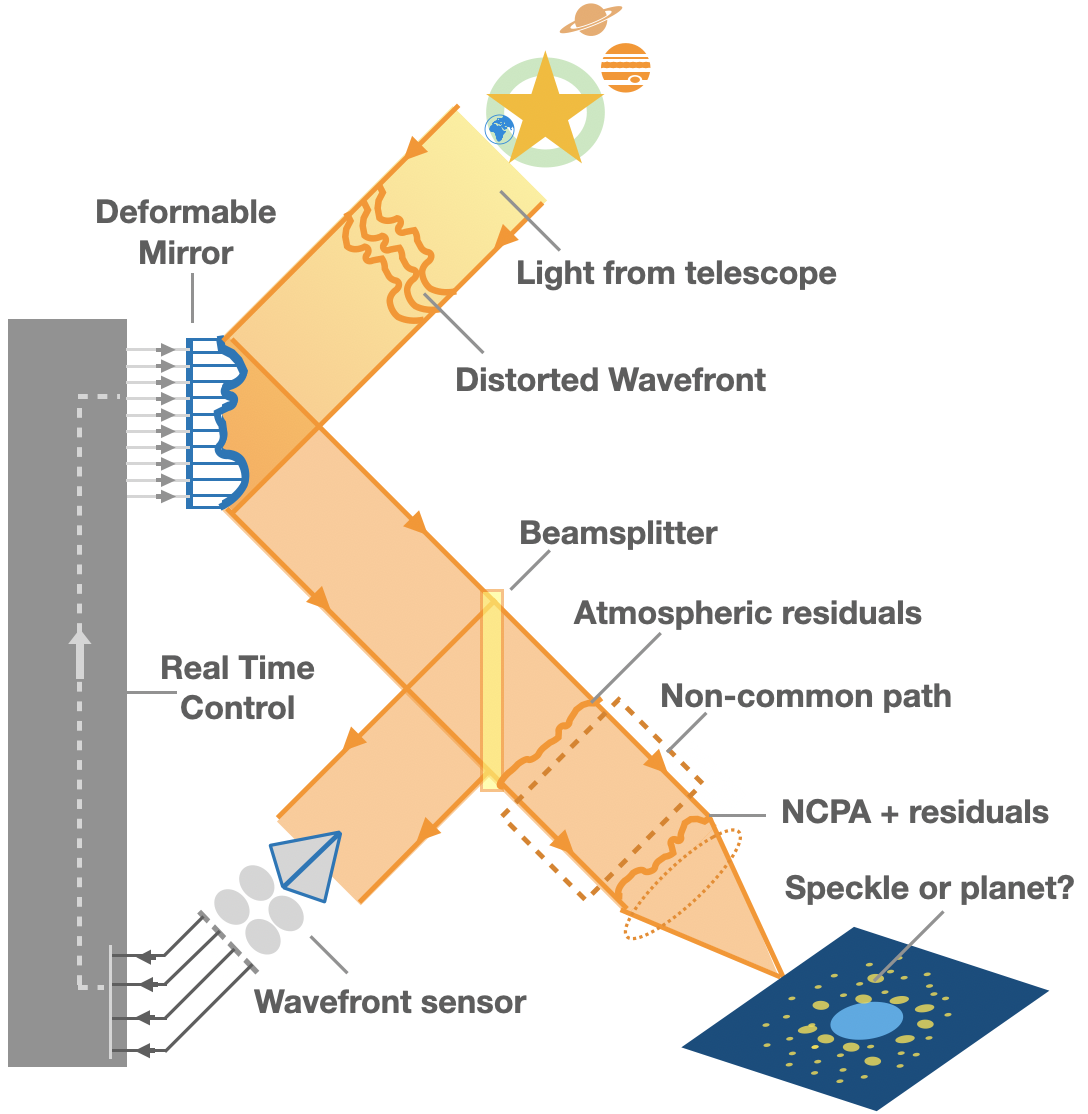
\includegraphics[width=0.45\textwidth]{fig/AO_schema.png}
\caption{Schematic view an AO system, presenting the problem of NCPAs, especially in the case of exoplanet imaging with a coronagraphic image.}
\label{fig:AO_schema}
\end{figure}



The causes for discrepancy listed above effects have timescales slower than the millisecond-level atmospheric turbulence timescale, and can be (nearly) static. 
In this paper, we refer to all discrepancies between WFS reference and optimal image wavefront as NCPAs, noting that in previous publications it usually only refers to optical defects non-common path aberrations.

 
NCPAs affect all AO systems, but are particularly acute in high contrast imaging where small wavefront errors can easily mask faint exoplanet images (cf Figure \ref{fig:AO_schema}). Furthermore, quasi-static aberrations do not average out to a spatially smooth halo as fast as the atmospheric speckles, leaving structures in the coronagraphic image which resemble planets, unlike speckles generated by the atmospheric turbulence alone.

%that could be subtracted in post-processing 
%\anthony{(not completely agree because ADI can partly deal with these, instead you should just say that they do not average as fast as the atmospheric speckles leaving wtructures in the coronagraphic image which resembles planets)}, unlike speckles generated by the atmospheric turbulence.

The most reliable approach to correct for NCPAs is to use focal plane images, ideally using the science detector. 
While several solutions have been suggested for static NCPAs \citep{vievardLAPD, Frazin2018,Vigan2018NCPA, BosFF2020, Potier2020darkhole}, the quasi static part remains a challenge to measure and compensate. 
%it remains an incompletely resolved issue 
%\anthony{too strong! I would rather say that these aberrations because they are not static but quasi static cannot be perfectly measured and compensated for}. 
%And quote techniques that can be used for that, with their pros and counts. (I'm thinking Phase diversity, Zernike asymetric pupil mask....)


%\cite{Esposito2015} have been pioneering the way to calibrate NCPAs with non-linear wavefront sensors, mainly PyWFS. 
%In fact, as they explain, 
In a closed loop AO system, NCPAs are usally compensated by subtracting a biasing reference signal
%must be corrected by introducing an offset 
in the WFS reference corresponding to the aberration to correct. Doing so requires good WFS response knowledge and stability, so that the adequate offset can be applied and maintained. This offset has to be updated on a daily or weekly basis, due to optical and mechanical variations in the instrument. Finding the adequate offset can be particularly challenging if the WFS exhibits non-linear response that must be accounted for, as is the case in some high-performance WFSs such as the Pyramid WFS (PyWFS) \citep{Esposito2020,Deo2019gain,Chambouleyron2020, Chambouleyron2021}.  

%They mainly solve the problem by adapting the optical gain with a tracking loop, thanks to a sinusoidal signal added on the DM, in order to have a modulation and a demodulation allowing to derive the value of the optical gain. \textit{to be confirmed, not sure to have understood well.}\\


%\anthony{(transition is not clear to me. how do we introduce the need for a new algo? ).}
In this paper we will present the DrWHO algorithm, a model-free focal plane wavefront sensing approach which is aimed at correcting slow and static wavefront aberrations, including the NCPAs, on a few seconds timescale. After stating the issues to be solved in Section \ref{sec:problem_statement}, we describe the algorithm in Section \ref{sec:algo_des}. Numerical simulations with the COMPASS software \citep{Compass} are presented in Section \ref{sec:compass}. 
%\anthony{(you have to present all the sections here in a more methodic way)}
In section \ref{sec:drwhoscexao} we show the results of the algorithm as obtained on sky with SCExAO.
%We introduced a metric to quantify the quality of the PSF, the flux concentration (FC), described in the same section.  %Anthony: too much details here.
Section \ref{sec:results} presents the main results of the on-sky validation, in terms of PSF and WFS reference evolution. In Section \ref{sec:Discussion}, we review the characteristics of the algorithm and describe further implications for use in HCI. 


%\textcolor{red}{Add more NCPAs methods?}




\section{Problem statement: What is a good WFS reference?}\label{sec:problem_statement}

%\subsection{\og{Fast and slow aberrations in the focal plane}{}}


%In xAO, a small error in the convergence point of the WFS can appear as a speckle that may be confused as a planet. 
%\og{The error budget of the PSF complex amplitude can be decomposed into 2 main components :}{}
%\begin{itemize}
%   \item \og{The fast aberrations - including the atmospheric residuals,}{}
%    \item \og{The static and slow aberrations - including the NCPAs described in Section \ref{sec:intro}.}{}
%\end{itemize}

%\og{The total WF phase arriving on the focal plane camera, $\Phi$ can be explicitly written as:}{}
%\begin{equation}
%    \og{\Phi = \Phi_{static/slow} + \Phi_{fast}}{} \\
    %\Phi = \Phi_{Residual} + \Phi_{NCPAs} +   \Phi_{LWE}
%     \label{eq:phase}
%\end{equation}


%\og{In the context of this paper, "fast" aberrations means "faster than NCPAs correction speed". The fast term is typically due to atmospheric turbulence not fully corrected by the AO system, while slow are due to the NCPAs. 
%This distinction is not critical to the algorithm described later, it is however helpful to understand which types of errors are addressed by it.}{}
%We include in the NCPAs term everything in the PSF path, which includes the errors induced from the optics, and the chromaticities of the wavefront. \\


%\nour{ to be moved in intro? :}
%\sout{One of the causes for slow wavefront errors that may not be fully compensated by the AO system is LWE, generating an island effect (IE) on the PSF. The LWE includes tip-tilt aberrations coupled with a differential piston - Delta P. This effect, notably due to the telescope spiders generating phase discontinuities of the wavefront, is seen by the 10-m class telescopes \citep{Milli_2018, BosFF2020}. 
%Measuring this effect is particularly challenging with a PyWFS, which gives a very week signal of the Delta P. \cite{ArielleSPIE2020} have demonstrated the incapacity of the PyWFS to measure this Delta P for the ELTs, in case of large $\frac{D}{r_0}$}. \\


In a closed loop AO system, each WFS measurement is compared to a WFS reference (usually by  subtraction after flux normalization), allowing to isolate residual wavefront errors that must be corrected by the DM. The resulting WFS signal is a representation
%, in WFS space, 
part of the closed-loop signal that remains to be corrected by the system deformable mirror (DM). The real-time control loop's function is to compute the DM offset that will compensate for these wavefront errors, thus bringing the WFS signal to where it gives a flat wavefront, such that the WFS reference defines the convergence point of the AO control loop.

 The WFS reference can be measured with an internal light source inside the instrument, before on-sky observations. This is done by averaging the WFS signal when taking a response matrix, corresponding to the WFS when there is no aberration induced. However, in reality, the \textit{ideal} WFS reference may be different from the internal source WFS reference due to optical illumination discrepancies. The WFS reference is also not static, constantly evolving due to quasi-static aberrations and wavefront chromaticity. The accurate calibration of the WFS is therefore a significant challenge for any AO system.
 %vincentc:cyou don't mention non-linearity, which is the real problem here !
 
%\og{ for various reasons (for example the light source may not be good enough to have internal-source calibrations, or there isn't a good optical reference that could be put in the system, or sometimes optics have distortion that change with time).}{} \\

Therefore, a continuous way to measure the \textit{ideal} reference is required for high accuracy wavefront correction. 
%This \textit{ideal} reference, Ref$^*$, is defined as follow:
%is defined such that it minimizes in terms of least square the following quantity:
%\begin{equation}
   %\| \mathbf{\Phi_{NCPA}} + \mathbf{\Phi_{Ref^*}}\|
%   \text{Ref}^* = argmin \| < \Phi_{target} > \|
%\end{equation}

%Where $\Phi_{target}$ is the phase \nour{qui engendre la tache de diffraction parfaite dans le rayon de correction - expliquer Phi target} at the focal plane, and where <.> is the statistical average over time.

%Where $\mathbf{\Phi_{NCPA}}$ is the phase of the NCPAs, and $\mathbf{\Phi_{Ref^*}}$ the phase of the \textit{ideal} reference, defined as Ref$^*$ = f($\pm \Phi_{NCPA}$), and f being the operator (corresponding to the response matrix in the case of a linear WFS) describing the WFS, taking wavefronts as input and providing WFS measurements as output. 

Finding this \textit{ideal} reference is particularly critical to xAO systems, where a slight deviation can introduce slow/static speckles that appear similar to a planet image.\\

%\og{To conclude, the \textit{actual} reference as set in the WFS is not the \textit{ideal} reference: the goal is to find what is the closest from it, and implement it on the WFS.}{}\\

%\og{However, besides the NCPAs, the atmospheric wavefront keeps evolving, therefore there are atmospheric residuals on top of the NCPAs seen by the focal plane camera, which measures a combination of the two. This makes the understanding of the \textit{ideal} reference more challenging as well as the NCPAs retrieval, since we can't differentiate which aberrations in the focal plane are due to the atmospheric residuals.  
%That implies that in the case of xAO instruments, the correction must be good enough so that the residual phase $\Phi_{Residual}$ is small enough for being able to sense the NCPAs, cf equation \ref{eq:phase}: if $\Phi_{Residual}$ >> $\Phi_{NCPAs}$, then $\Phi_{Residual} \sim \Phi$.}{}

%\og{The DrWHO algorithm, described in Section \ref{sec:algo_des}, aims at finding, then applying, this \textit{ideal} reference, by measuring in a continuous way what is the closest from this \textit{ideal} reference, given there are remaining atmospheric residuals making it more challenging. After a few iterations of the algorithm, the goal is to be able to extract this \textit{ideal} reference, and thus converge towards a compensation of the slow and static aberrations.}{} \\




\section{Algorithm description}\label{sec:algo_des}
%\textcolor{blue}{Anthony: La section suivante doit decrire l'algo, et il faut qu'on comprenne a ce stade "le pourquoi" de ces etapes. A la fin de la 3 ce qui doit manquer au lecteur c'est les resultats mais il doit etre en mesure de comprendre pourquoi tu procède comme ca (au moins de facon globale, les details peuvent etre compris ensuite). Il faut pouvoir expliquer pourquoi 30s de moyenne et pourquoi 10\%, est ce qu'il s'agit de guess, de valeurs optimales... et il faut expliquer comment tu arrives à ces specifications.\\}

Since the goal is to ensure the AO loop converges to the \textit{ideal} reference, the \textit{actual} reference should be updated continuously. To do so, DrWHO regularly re-estimates this reference, chosen by selecting the WFS images corresponding to best PSF image quality. The algorithm is thus a lucky imaging of the PSF leading to the selection of the best WFS images. \\
The quality criteria (\emph{score} hereafter) for the PSF is flexible: it can be SR, contrast, minimum of intensity, etc. The algorithm proceeds as follows: on a defined timescale (set arbitrarily at 30 seconds), the algorithm first selects the best PSF frames according to a score metric and a predefined selection fraction (arbitrarily set to 10\%). Then, out of those 10\% frames, the corresponding WFS raw frames are extracted from the AO telemetry and averaged; the resulting WFS frame replaces the WFS \textit{actual} reference, and the algorithm is iterated to continuously optimize the WFS reference. \\

%\anthony{I'm not completely sure to understand the assumptions here.... to be discussed "de vive voix"}

As the algorithm proceeds, the AO loop point of convergence removes NCPAs and other slow aberrations. Thus, the PSF quality improves, and converges towards a better score. 
We present the procedure step by step of DrWHO with the  description in algorithm \ref{algo:DrWHO}, and a schematic view of the algorithm is in Figure \ref{fig:DrWHOschema}.\\


\begin{algorithm}
 \KwData{\begin{itemize}[noitemsep,nolistsep]
     \item WFS frames
     \item fast science camera frames
 \end{itemize}}
 \KwResult{Update the reference of the WFS}
 \textbf{Initialization:} take the reference of the WFS with the internal light source\;
 \While{AO loop is running}{
 \begin{itemize}
     \item acquire WFS and fast science images\;
    \While {DrWHO iteration (30 s) is running} {
    \begin{itemize}
        \item take the 10\% best science data\;
        \item take the corresponding WFS images\;
        \item average them, weighted on the score value\;
        \item the resulting frame replaces the WFS \\
        reference\;
        \item WFS reference updated. 
    \end{itemize}
   }
   \item restart DrWHO iteration
   \end{itemize}
   Change of AO point of convergence;
  }
 \caption{DrWHO algorithm mindset}
 \label{algo:DrWHO}
\end{algorithm}


%Therefore, our reference $\overrightarrow{r}$ should be the sum of the best PyWFS measurements $\overrightarrow{s_{best}}$ contributors so that we can write  $\overrightarrow{r} = \sum_{i=1}^{N} a_i \overrightarrow{s_{best}}_i$, with each of the $\overrightarrow{s_{best}}_i$ being the best PyWFS measurements, ans the $a_i$ being the coefficient for the weighted average.

\begin{figure*}[t]
\begin{center}
\centering
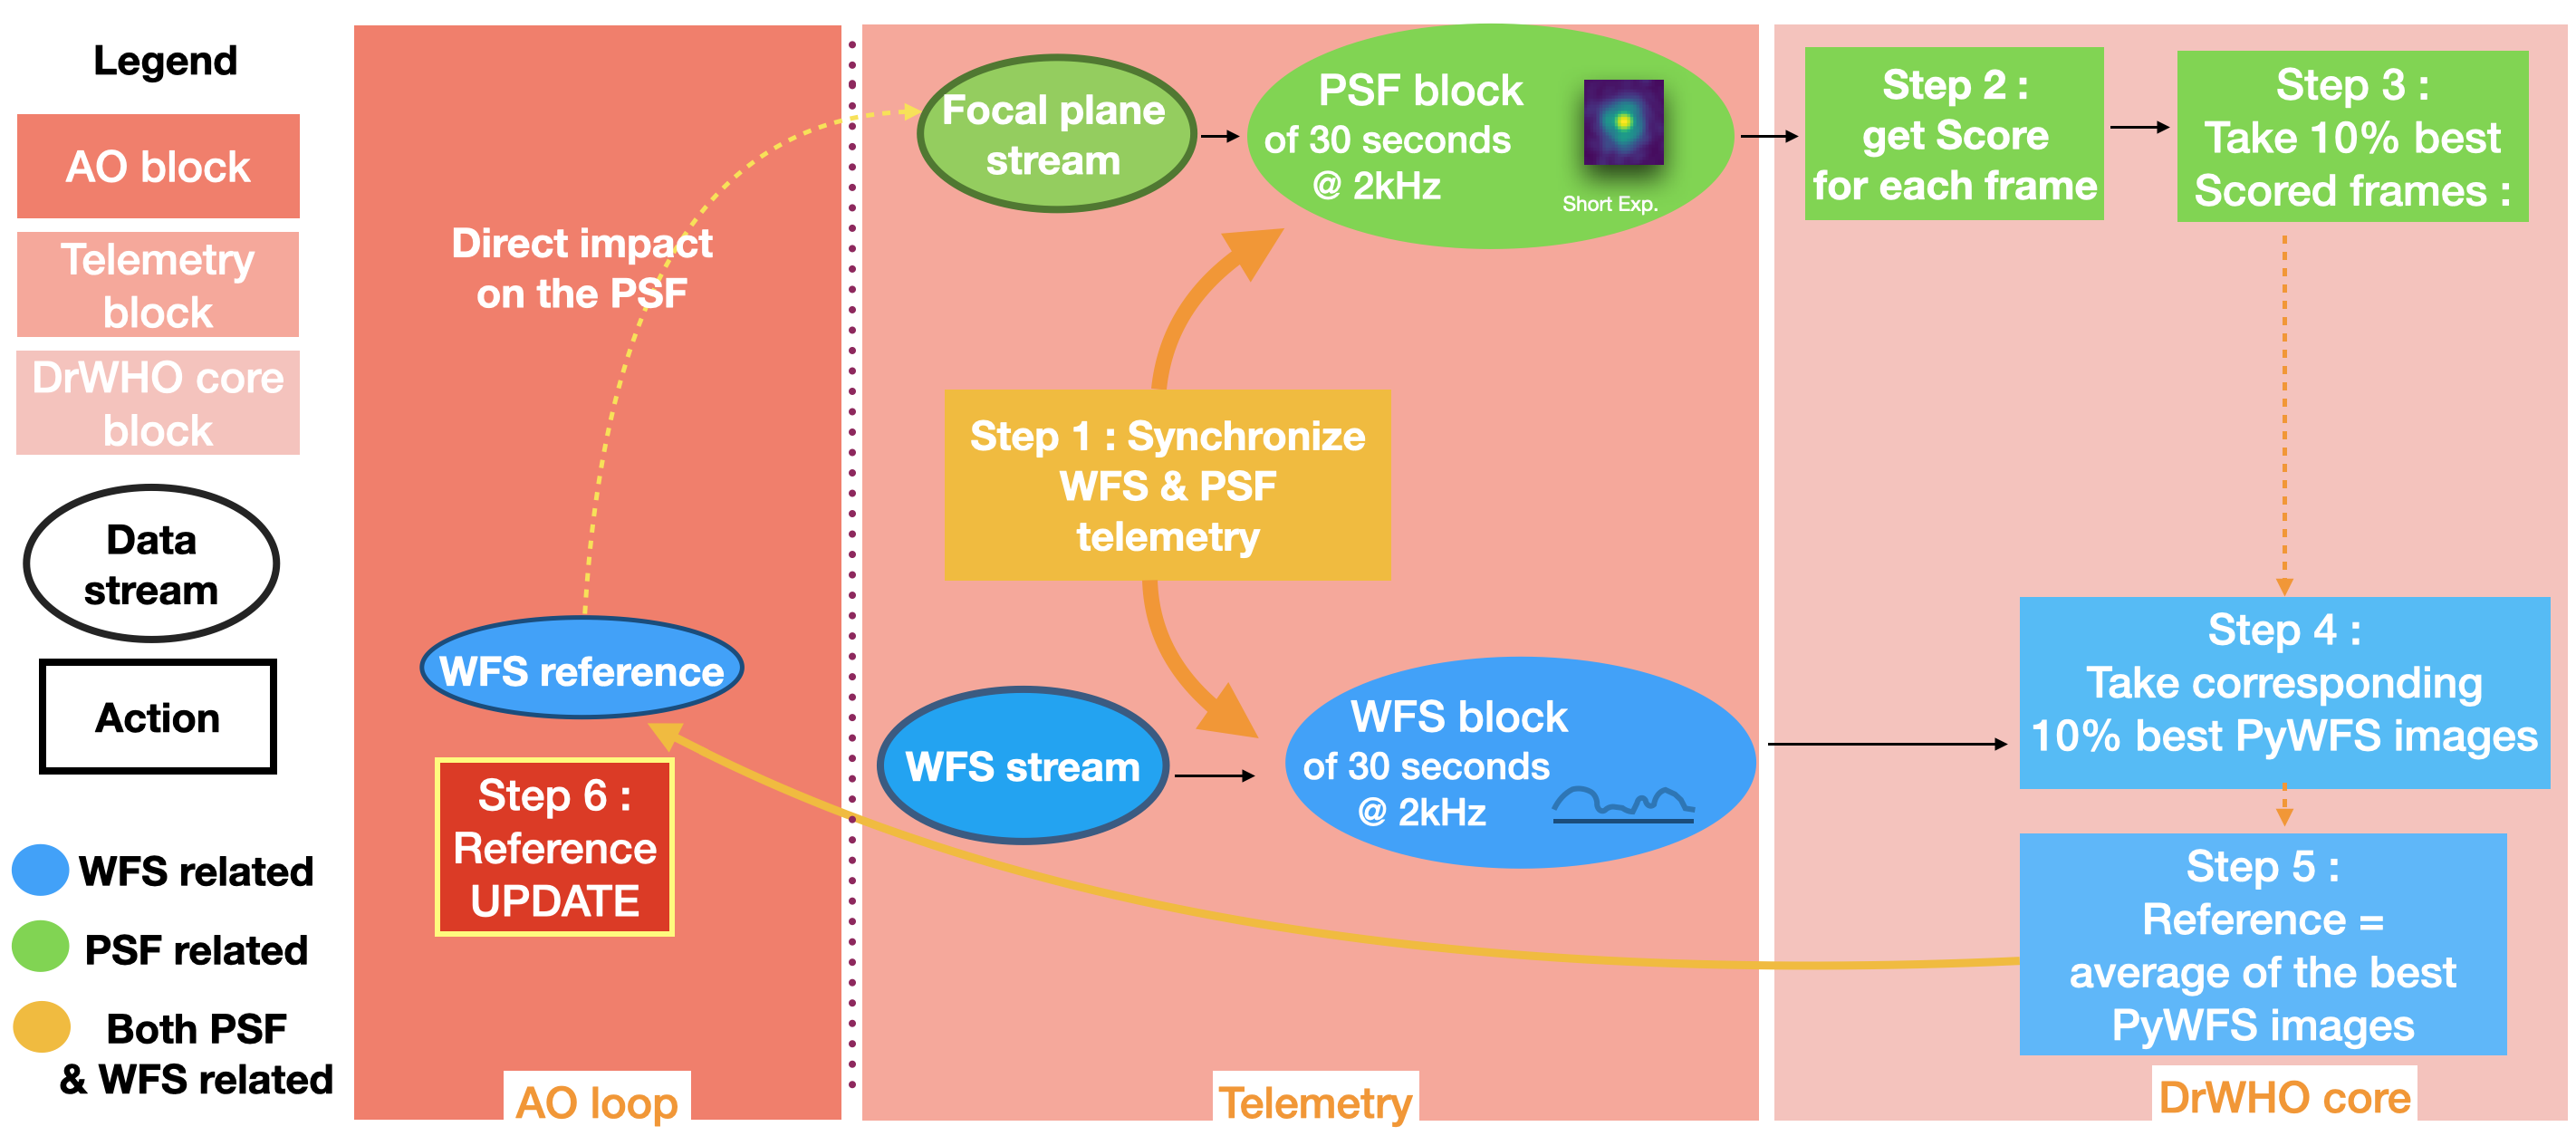
\includegraphics[width=0.95\textwidth]{fig/DrWHOschematicview.png}
\caption{Schematic view of DrWHO. From left to right, as the AO loop is running, the PSF and WFS telemetry are acquired. These data streams are then synchronised and re-sampled to the same timescale, here spanning the length of the DrWHO iteration which we set at 30 seconds (cf \ref{sec:syncdata} for deeper explanations). On the PSF data cube, the second step of DrWHO is to compute the score for each frame. The following step is to select a fraction (10\%) of the best PSF according to the quality criteria. The 4th step is to take the corresponding WFS images, then (5th) to average them to make one single PyWFS image : this corresponds to the new reference for the iteration. Finally, the 6th and final step is to apply this new reference to the PyWFS, and thus update it. This last step is the only one not transparent to the AO loop, as it changes its point of convergence.}
\label{fig:DrWHOschema}
\end{center}
\end{figure*}

%This can be approximated as a kind of very simplistic reinforcement learning approach, as shown in Figure \ref{fig:DrWHO_RL}.  The agent is here the algorithm DrWHO, the environment is the PSF, the reward is the SR, and the action is the WFS reference update. The policy used as described earlier is a simple binary selection of the PSFs, based on lucky imaging.\\

%\begin{figure*}[t]
%\begin{center}
%\centering
%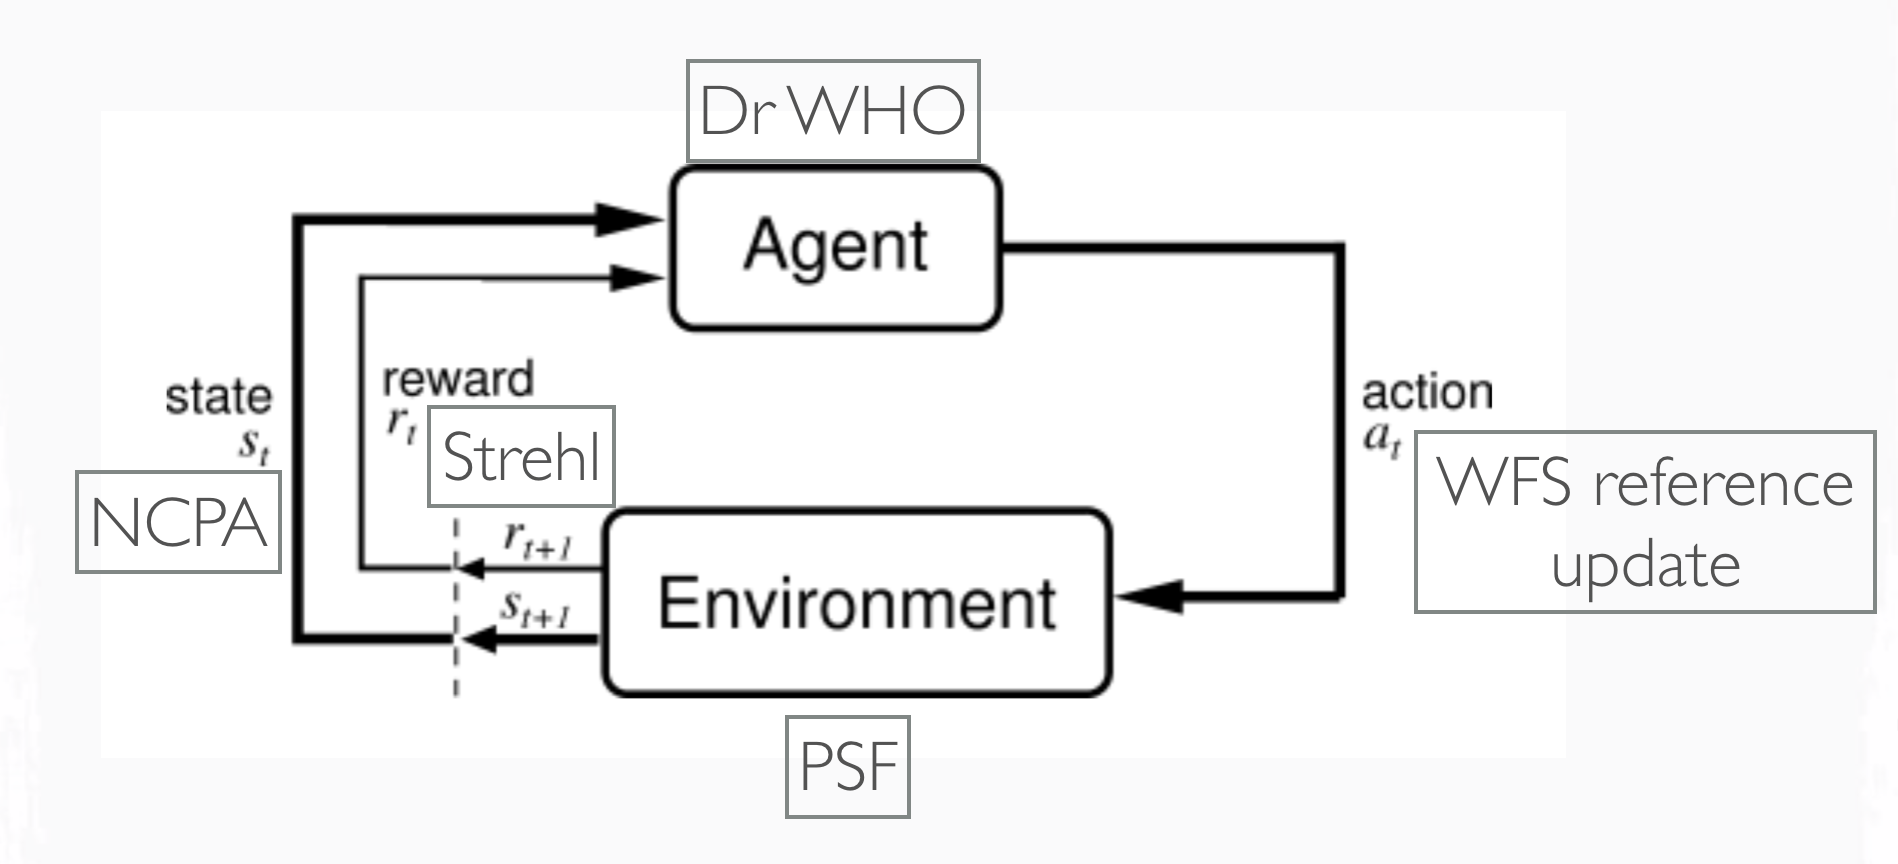
\includegraphics[width=0.4\textwidth]{fig/DrWHO_RL.png}
%\caption{Simplistic reinforcement learning description of DrWHO.}
%\label{fig:DrWHO_RL}
%\end{center}
%\end{figure*}



\section{Validation via numerical simulations}\label{sec:compass}

This section presents the AO simulation set up with the COMPASS simulator \citep{Compass}.
COMPASS is a versatile AO simulator, which has been designed to meet the need of high-performance for the simulation of AO systems, modeling several kinds of AO features, including several types of WFS, atmospheric simulations, DMs, telescopes, and RTCs. It offers a suitable environment for simulating Single Conjugate Adaptive Optics (SCAO), for Very Large Telescopes (VLT) and Extremely Large Telescopes (ELT) as described in \citet{Vidal2018}.  Simulations of DrWHO on the COMPASS software have first been implemented to explore the algorithm feasibility and potential. 

%and implement it first in simulation ahead of implementations on the bench of the SCExAO instrument, with the internal light source, and before the observations. Being able to go back and forth between simulation and instrument have help pin down the issues faced.  \\

\subsection{Extreme AO simulation}

The first step was to simulate an xAO on COMPASS. We looked for simulating an AO close to the SCExAO instrument, including the pre-correction of the first stage of the AO. The high contrast instrument on the Subaru Telescope is composed of two AO systems, AO188 \citep{AO188_minowa}, and then SCExAO. AO188 is the low order first stage AO system, with a curvature wavefront sensor and a 188-actuator DM. SCExAO has a much higher capacity to correct higher orders of aberrations, with a Pyramid WFS (PyWFS) and a DM of 45 actuators across the beam diameter. \\

%\og{Regarding the PyWFS, the WFS concept has first been introduced in 1996 \citep{Ragazzoni1996}, and has the precious characteristic of being particularly sensitive in regard to photon noise, comparably to the other kind of WFSs. It took nearly a decade before its first use in astronomy, with its first implementation in a very large telescope, the Large Binocular Telescope (2x8.4m) in 2010 \citep{Esposito2010LBT}. Now, the PyWFS is already implemented on sky on several 8-10 meter class telescopes, and has been the design choice of the first light instruments of all the ELTs. However, the PyWFS linearity and calibration issues remain an active field of research \citep{Deo2019gain, Chambouleyron2020, ArielleSPIE2020, Esposito2020}. The PyWFS non-linearities are non-trivial to model, so far approximations to describe the difference of sensitivity between the lab and on-sky are described by optical gains, which is a coefficient, smaller than one, describing the sensitivity ratio.}{} \\

%\sout{The Pyramid wavefront sensor (PyWFS), introduced in 1996 \citep{Ragazzoni1996}, has the precious characteristic of being particularly sensitive in regard to photon noise, comparably to the other kind of WFSs. It took nearly a decade before its first use in astronomy, with its first implementation in a very large telescope, the Large Binocular Telescope (2x8.4m) in 2010 \citep{Esposito2010LBT}. Now, the PyWFS is already implemented on sky on several 8-10 meter class telescopes, and has been the design choice of the first light instruments of all the ELTs. However, the PyWFS linearity and calibration issues remain an active field of research \citep{Deo2019gain, Chambouleyron2020, ArielleSPIE2020, Esposito2020}.}
%\nour{a pomper sur le papier de vincent}

Reproducing exactly SCExAO on COMPASS has not been the primary focus of this experiment, but rather to have a simulation that is close enough to be relevant for testing the algorithm, and predict results on SCExAO. Table \ref{tab:simuParams} synthetizes the parameters used in the COMPASS simulations.\\



\begin{table}[t]
		\centering
		\caption{%
			AO numerical simulations parameters.
		}
		\label{tab:simuParams}
		
		\renewcommand{\arraystretch}{1.2}
		\begin{tabular}{ll}
			\multicolumn{2}{c}{\textbf{Numerical simulation configuration}}\\
			\hline\hline
			\multirow{4}{*}{Telescope} & $D$ = 8.~m diameter\\
			& Subaru pupil \\
			& $\quad$No support spiders\\
			& Central Obstruction = 0.12 \\
			\hline
			\multirow{5}{*}{Turbulence layer} & von Kármán, ground layer only\\
			& $r_0$ = 0.16 at 500~nm \\ % variable in a\\
			%& $\quad$useful range of 7.0 - 35.0~cm\\
			& L$_0$ = 20~m\footnote{to simulate AO188's pre-correction}, \\
			& $||\overrightarrow{\mathbf{v}}||$ = 10~m.s$^{-1}$\\
			\hline
			PyWFS & \\
			$\quad$Subapertures & 64$\times$64 \\%-- pixel size 42~cm.\\
			%& 24,080 useful pixels\\
			$\quad$Wavelength & Monochromatic, 750~nm\\
			$\quad$Throughput & 50\% \\
			$\quad$Modulation & Circular, 3~$\frac{\lambda}{D}$ radius, 24 points\\
			$\quad$Photon noise only \\% & 0.3~$e^{-}$\\
			\hline
			Deformable mirror & \\ 
			& 48 actuators on the diameter\\
			\hline
			Focal Plane Camera & \\
			$\quad$Wavelength & Monochromatic, 1.65~$\mu$m\\ 
			$\quad$Photon noise only \\
			%\hline 
			%Source & On-axis natural guide star\\
			%Guide star flux & Zero point: $2.6 \times 10^{10}$~ph.s$^{-1}$.m$^{-2}$\\
			%\hline
			%\multirow{5}{*}{Adaptive mirrors} & Tip-tilt mirror\\
			%& Hexagonal M4 model pattern\\
			%& $\quad$Pitch of 54~cm\\
			%& $\quad$Coupling of 0.24\\
			%& $\quad$4,310 controlled actuators\\
			%& Both with infinite bandwidth\\
			\hline
			RTC controller & \\
			$\quad$Loop rate & 2~kHz\\
			$\quad$Method & Linear modal integrator\\
			%$\quad$Latency & Data flow 1 frame + MVM 1 frame\\
			$\quad$Basis & DM Karhunen-Loève (KL) basis\tablefootmark{(a)} \\
			$\quad$Loop gain & 0.3\\
			$\quad$Controlled modes & 1505\\
			$\quad$Modes filtered & 300\\
			\hline
		\end{tabular}
		\tablefoot{
			\tablefoottext{a}{- \cite{Compass}}
		}
	\end{table}

The simulation is idealized, with no source of noise other than only the photon noise on both the WFS and the science detector, and does not take into consideration the telescope spiders. Furthermore, we considered a PyWFS with a higher sampling than on the SCExAO instrument (64 versus 50 \nour{pixels over the PyWFS diameter}), hence higher performance than achieved on-sky. The PyWFS is working in the visible at 750~nm, and the detector in the infrared at 1650~nm (cf Table \ref{tab:simuParams}). Finally, the COMPASS simulation allows to have synchronized exposure times, which is not the case on SCExAO (cf Section \ref{sec:syncdata}).  
%\nour{We did not perform any compensation of the modal gains on the WFS.}
%The simulation of SCExAO on COMPASS is therefore overall optimistic in terms of AO performance. 
The quality criteria used for quantifying the PSF on COMPASS is the SR. 


\subsection{DrWHO on COMPASS}
We implemented the DrWHO algorithm as described in algorithm \ref{algo:DrWHO} and Figure \ref{fig:DrWHOschema}. Results are presented for a case with 15 DrWHO iterations, each having 10 000 AO loop iterations (corresponding to 5 seconds at 2kHz). The number of AO loop per DrWHO iteration was constrained by the simulation time. 

%\textcolor{red}{mettre en exergue le temps de simulation étant une contrainte, because of simulation time, I used 5 seconds instead of 30 seconds. demonstration de principe}

NCPAs, corresponding to a linear combination of the first 12 Karhunen-Loève modes (which is the modal basis used for computing the response matrix), with randomized amplitude RMS, were applied on the science path (not visible to the WFS), with a total amplitude of 30~nm RMS (cf Figure \ref{fig:NCPAs_psf}. Such amplitude for the NCPAs is slightly greater than what is expected in reality. In fact, on SCExAO, NCPAs are expected to be of approximately 20~nm.


%\nour{\textbf{NB:} We decided to go for a relatively realistic simulation of the SCExAO system, with a small amount of NCPAs. Keeping small NCPAs prevents from heavily impacting the SR, which would have been useful for better understanding the NCPAs correction of the algorithm, however it allows us to ignore the corrections of the optical gain, which is out of the scope of this paper. }

On SCExAO, and on most systems, the impact of the NCPAs over the SR is relatively small, therefore it is not the best metric to quantify the efficiency of the algorithm, as the AO is dominated by dynamic wavefront errors. In fact, NCPAs are problematic for HCI since they add quasi-static features to the PSF. However, the SR it is a good metric to make sure the algorithm does not diverge, in particular through the high-order modes as they could adopt a random walk behavior.


Table \ref{tab:compass_comp} presents the SR for different cases: when the loop is running without NCPAs, the SR is of 87.9\% at 1.65 $\textmu$m. When adding the NCPAs, without compensating them yet,  the SR drops to 86.8\%. Figure \ref{fig:NCPAs_psf} shows the impact of the NCPAs on a PSF free of other aberrations. 

\begin{figure}[t]
\begin{center}
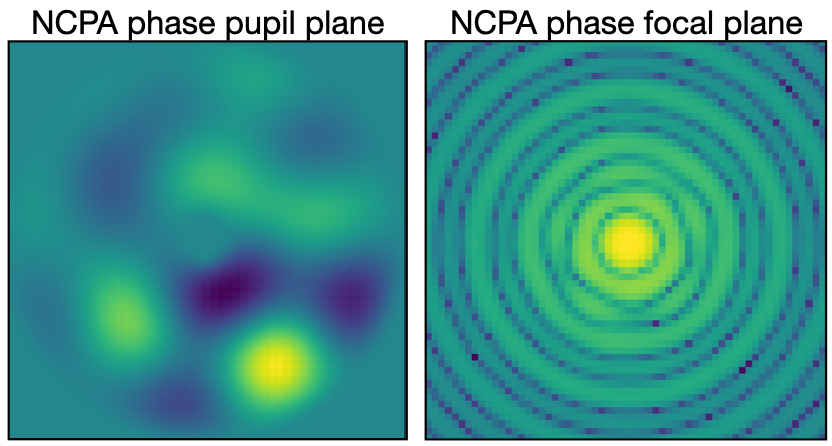
\includegraphics[width=0.4\textwidth]{fig/NCPA_compass.png}
\caption{Left: phase of the NCPAs in the pupil plane, with an amplitude of 30~nm RMS. Right: Corresponding PSF of size 60x60 pixels \textcolor{red}{talk in field of view not pixels}, at 750~nm.}
\label{fig:NCPAs_psf}
\end{center}
\end{figure}



\subsection{Simulation results}
\subsubsection{Results in terms of PSF quality}

\begin{table}[]
\begin{tabular}{l|ccc}
                               & \multicolumn{1}{l}{No NCPAs} & \multicolumn{1}{l}{with NCPAs} & \multicolumn{1}{l}{with DrWHO} \\ \hline
SR LE (\%)                          & 87.9                      & 86.8                         & 87.7                           \\
$\sigma_{OPD}$ (nm RMS) & 94.3                      & 98.8                         & 95.1                         
\end{tabular}
\caption{Comparison of the long exposure (LE) Strehl ratio between the following cases of the AO loop: no NCPAs, NCPAs alone, and post DrWHO with the NCPAs. The second line corresponds to the RMS of the wavefront for each of those cases, calculated from the SR of the line above with the Maréchal approximation.}
\label{tab:compass_comp}
\end{table}


Figure \ref{fig:compass_LE_SR} and Table \ref{tab:compass_comp} presents the result of the SR after the DrWHO run: the final SR after the 15 iteration DrWHO run reaches 87.7\%, for a maximum of 87.9\%. As Figure \ref{fig:compass_LE_SR} displays it, nearly half of the SR improvement is obtained within the first iteration of DrWHO. Then, the SR keeps slowly improving, until it reaches a plateau. After the run of 15 iterations, the SR has improved of 1.1\%. \\

In order to better understand the impact on the optical path difference (OPD), we used the Maréchal approximation:
%stating that the SR can be linked to the variance of the phase through the following formula :
\begin{equation}
    \text{SR} = \exp(-\sigma_{\Phi}^2) = \exp\left(%
    -\dfrac{4\pi \sigma_{\text{OPD}}^2}{\lambda^2}
    \right)
\end{equation}

The corresponding values for $\sigma_{OPD}$, calculated from the measured SR, can be found in Table \ref{tab:compass_comp}. The values allow to estimate the total compensation in nm RMS, by calculating the quadratic difference of the  $\sigma_{OPD}$ before and after the DrWHO run, which corresponds to a total of \textbf{26.6~nm}, which corresponds to 89\% of the total amplitude of the NCPA, 30~nm RMS.\\


\begin{figure}[t]
\begin{center}
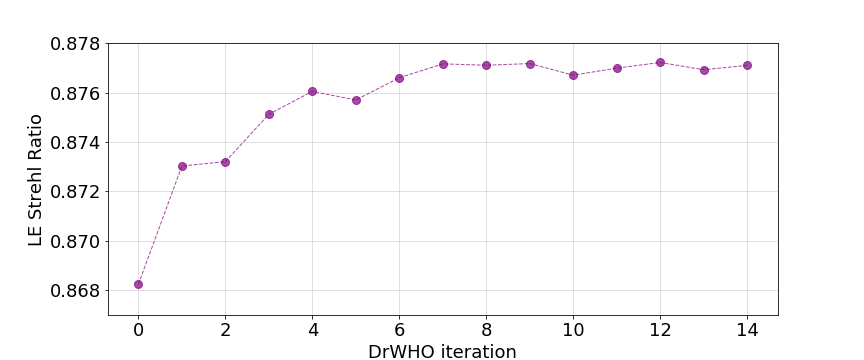
\includegraphics[width=0.52\textwidth]{fig/LE_SR.png}
\caption{Evolution of the long exposure (LE) Strehl ratio during the DrWHO run on COMPASS, corresponding to 15 DrWHO iterations of 10 000 AO loop each.}
\label{fig:compass_LE_SR}
\end{center}
\end{figure}



%NB : What is most likely happening is that the std of the wavefront residuals is much smaller than the quantity of the NCPAs (100nm), that are covering only the first 10 Zernike modes after tip-tilt. Thus we are likely fixing those 10 modes very quickly, but we are adding a mess with the higher order modes, because of the statistic of the selection. \\
%A way to go around this issue would be to decrease the selection fraction as DrWHO iterations proceeds, from a high percentage of selection of best images at first, to a small percentage of selection with an integrator filter then. \\


\subsubsection{Results in term of modes corrected}

The 15 references for each iteration of the DrWHO run were projected over the modal basis with which the response matrix was acquired. Figure \ref{fig:ho_modes} shows this modal decomposition along with the ideal NCPAs correction (opposite of NCPAs modal coefficients), where the opposite of the NCPAs\footnote{(-1)*NCPA} was added, to better compare the correction. It appears from the top plot of this figure that, as we previously concluded, the algorithm converges from the first iteration towards a compensation of the NCPAs. The average of all those references (minus the reference 0, which is the initial reference) is neighbouring the NCPAs aberrations. This proves that DrWHO measured them, with the right amplitude, and compensated for them. 
The middle and bottom plots of this figure prove that the algorithm does not diverge at the higher order modes, as suggested by the increase of SR. 
The quadratic sum of 12 modes from the mean of all the references from the algorithm corresponds to \textbf{36~nm} RMS, which is roughly consistent with the amplitude of the NCPAs.


\begin{figure}[t]
\begin{center}
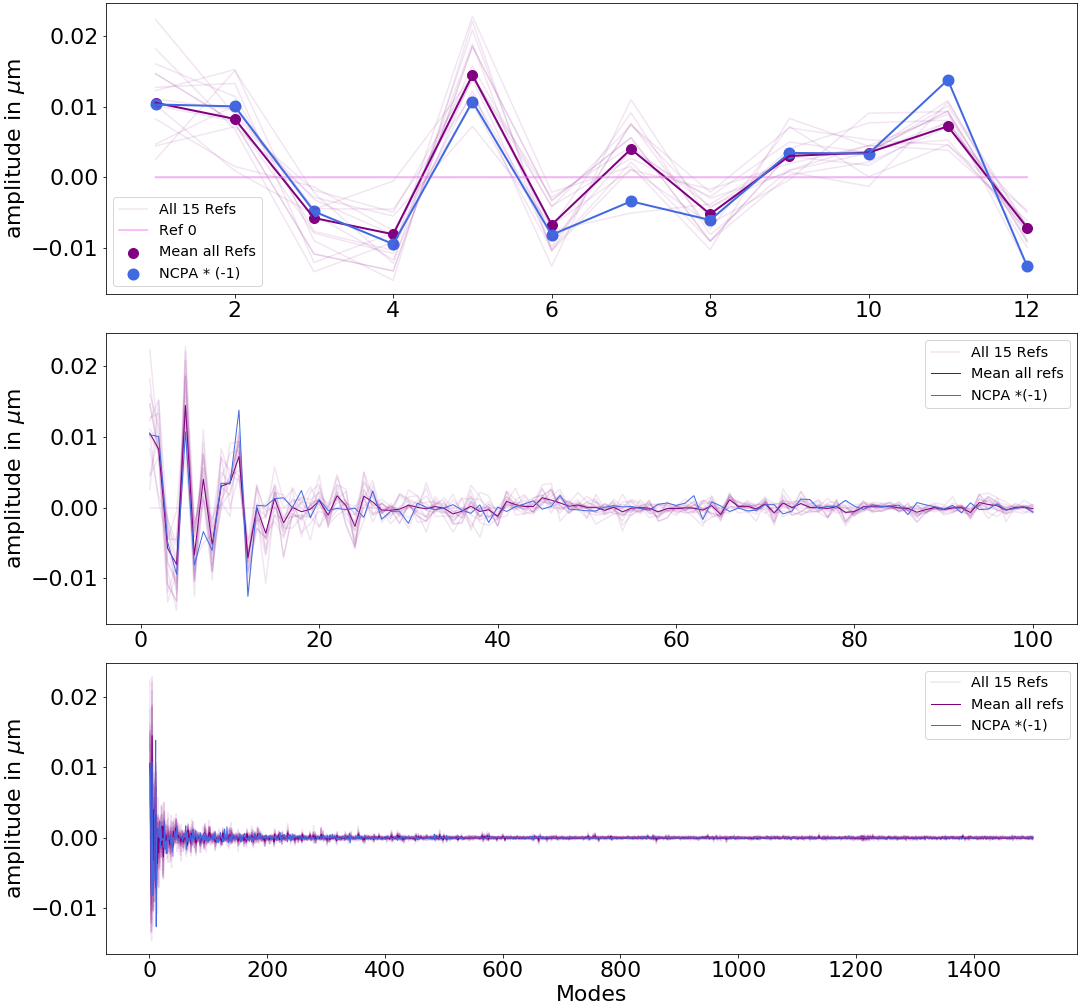
\includegraphics[width=0.47\textwidth]{fig/ho_modes.png}
\caption{Top: projection of the references provided by the 15-iteration DrWHO run over the modal basis, with the projection of the opposite of the NCPAs, in order to better visualise the correction. Middle: projection over the first 100 modes. Bottom: projection over all the 1505 modes.}
\label{fig:ho_modes}
\end{center}
\end{figure}

\subsubsection{Discussion}
DrWHO on COMPASS improved the image quality in terms of SR, and the NCPAs applied over the PSF, unseen by the WFS, were almost totally corrected. Half of the correction has occurred at the first iteration of the algorithm. The projection of the references from DrWHO is showing that the NCPAs are nearly entirely compensated for, and the higher orders, where we did not apply NCPAs, are not diverging. 
However close we got from the SR without NCPAs, we did not reach the original pre-NCPAs SR. Besides the fact that SRs are defined up to a certain precision only \citep{Roberts2004Strehl}, this can be explained by two effects: first, as seen in Figure \ref{fig:ho_modes}, the modes are not perfectly compensated; and second, the modes of the references beyond the ones applied on the NCPAs (12 modes) did have a small -yet not fully negligible- impact on the reference update, hence they may have slightly impacted the SR.\\



\section{DrWHO on SCExAO}\label{sec:drwhoscexao}


The DrWHO algorithm was then adapted and deployed on the SCExAO instrument, which is located on the infrared Nasmyth platform of the Subaru Telescope, downstream of the AO188 instrument. Several aspects are different between the COMPASS simulation and the SCExAO instrument, however the concept remains the same.

The instrument is equipped with a Pyramid WFS operating in the 600-950~nm wavelength range \citep{Lozi2019PWFS}. The real time control (RTC) of the AO system is managed by the CACAO software - Compute And Control for Adaptive Optics - \citep{cacao2018}. The DM has 45 actuators across the active pupil, giving a control radius of 22.5$\lambda$/D. We use the CACAO software to interact with the system and implement the algorithm, to communicate between the PyWFS and the DM.
%CACAO provides 12 different DM control channels, on which several corrections are implemented from additional wavefront sensors or wavefront control techniques \citep{BosFF2020}.
%Furthermore, CACAO updates the reference of the PyWFS by adding an offset which prevents the AO loop to cancel out the commands of the wavefront control sensing techniques with the DM. 
There are several scientific cameras downstream SCExAO. The one used for this paper was the VAMPIRES camera, which operates in the visible \citep{vampires2015}, with a pixel scale of 6.1~mas of field of view. 

\begin{figure*}[t]
\begin{center}
\centering
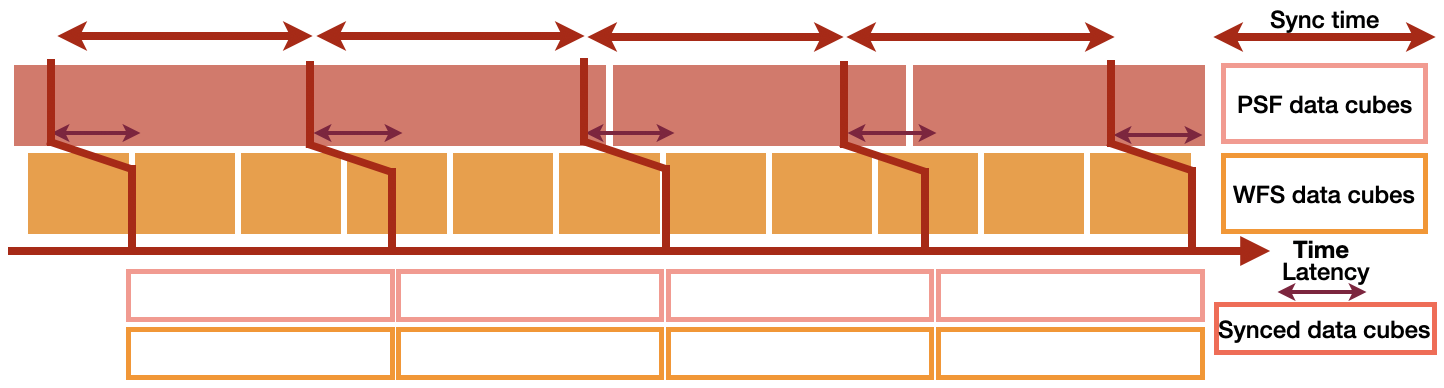
\includegraphics[width=0.8\textwidth]{fig/sync_image.png}
\caption{Schematic view of how the synchronization of files works. Given two data streams with a known latency between them, the algorithm generates two synchronized files for those data.}
\label{fig:sync_files}
\end{center}
\end{figure*}

\subsection{Data synchronization and re-sampling}\label{sec:syncdata}

On SCExAO, the PyWFS and the short exposure focal plane camera run at different frequencies, hence the need of synchronising the data streams to run DrWHO. 
This is done directly on the telemetry files that are saved to the file system, but not in real time. Indeed, DrWHO needs frames to be synchronized but not precisely in real time, since one iteration of the algorithm is several seconds long. 
A script for telemetry synchronization is has been implemented, to which four inputs are required: 
\begin{itemize}
    \item the PyWFS data telemetry timeseries;
    \item the focal plane camera data stream;
    \item absolute timestamps of each exposure on both timeseries, retrieved from a hardware latency calibration process 
    \item the output sampling frame rate
\end{itemize}

For example, if the focal plane camera runs at 1kHz, the PyWFS camera runs at 2kHz, and a 3kHz output frame rate is requested, both input streams will be resampled to a common 3 kHz frame rate. Once launched, the synchronization script waits for data cubes (FITS files) and the corresponding timing files to appear on the hard drive, reads them and re-samples them to the same time baseline. This script handles differential latency between the streams, potential missed frames, and possible interruptions in the input streams acquisition. A linear interpolation is performed to re-sample input streams to output data cubes.
This script provides output data cubes of the required length (which is an input parameter of the script), that are saved on the file system. As described  above, the operation is not real-time as files need to appear to generate the re-sampling. Choosing the length of the data cubes is linked with the latency we need for DrWHO. The script needs to be started once only, then it catches up as the AO loop is running. Figure \ref{fig:sync_files} gives a visual explanation of this file synchronization.




\subsection{PSF quality criteria}
%The quality criteria for quantifying the PSF on SCExAO isn't an obvious choice. 
%\textcolor{red}{expliquer qu'on a utilisé le strehl sur simu, parce qu'on peut le convertir en OPD. en vrai, c'est tres compliqué de mesurer le strehl (roberts 2004) d'ou la necessité d'introduire le FC.}\\

The SR is rather complicated to measure on real PSFs, and is often not reliable \citep{Roberts2004Strehl}. Hence, we felt the need of a different quality criterion. 
We introduce the Flux Concentration (FC), which is the $\alpha$-norm defined as: 
\begin{equation}
\centering
    \text{FC} = \frac{\sum_i  (x_i^{\alpha})}{ (\sum_i x_i ) ^{\alpha}}
\end{equation}



%With  $\| PSF \|$ being the PSF image, $\| PSF_{o} \|$ the ideal PSF image,
With $x$ being the pixel value, and $\alpha > 0$. If some pixels have a negative value following a dark subtraction due to photon noise, then the pixel value is set to zero. 
This quantity is independent of the total flux, it simply describes the flux concentration. It may be compared to a SR, with the difference that the Strehl only considers the peak value, while FC considers all pixels making it more robust against measurement noise and pixel sampling effects.  \\
If the intensity is concentrated in one pixel, FC equals 1. For the intensity spread over several pixels, FC < 1. If the light is equally spread over the pixels, then FC tends to 0. 
\\

We will be using $\alpha = 2$, noting that higher values of $\alpha$ favors the brightest pixels. \\

We choose to compute FC for a subarray of the full image covering the central region of the PSF, in order to focus on the low order modes: wavefront aberrations at low spatial frequencies (except for Tip-Tilt) redistribute the flux in such a way that it spreads across more pixels in the central region of the PSF, and thus the higher the low order aberrations will be, the lower the FC will get. 
The FC can be normalised by the FC of a simulated perfect PSF - which we will call 
FC$_0$ - 
computed for the pupil of the telescope (cf Figure \ref{fig:perfect_psf}), as the FC is a relative number. 
This new quantity is referred to as the normalized FC (nFC): nFC = FC / FC$_0$.


\begin{figure}[t]
\centering
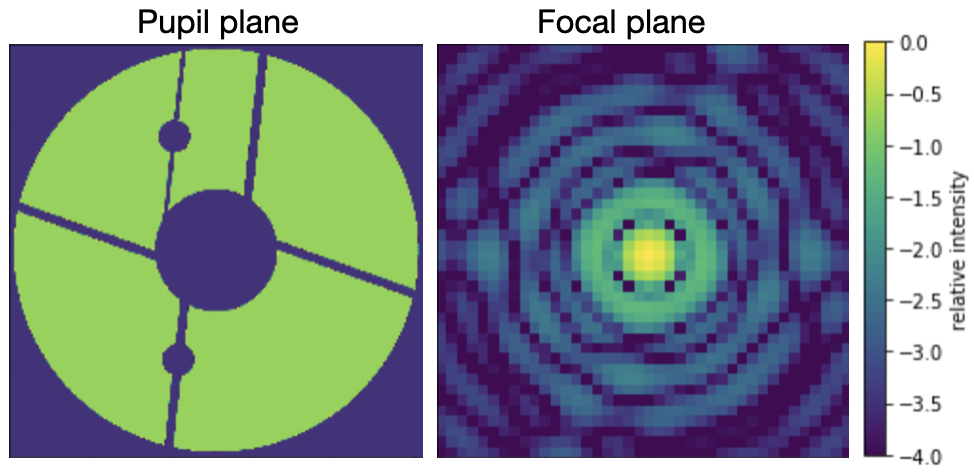
\includegraphics[width=0.32\textwidth]{fig/perfect_psf.png}
\caption{Left: simulated pupil plane, including the spiders and a mask for two dead actuators. Right: simulated perfect SCExAO PSF matching the wavelength, field of view and orientation of Figure \ref{fig:SkyResult} shown in logarithmic brightness scale. }
\label{fig:perfect_psf}
\end{figure}

\section{On-sky results}\label{sec:results}



\subsection{Observation setup}

We performed observations on the night of December 8 UT, 2020, during which we ran DrWHO over a period of 10 minutes, corresponding to 20 iterations of 30 seconds. Each iteration entails synchronized data cubes of 29939 frames for both VAMPIRES and PyWFS images. The observation conditions at that time were a seeing of 0.5", and a wind speed of 4 m/s. The observed target was the $\xi$ Leo star, at an airmass of 1.03. The window size of the image for the selection of the quality criteria was of 70x70 pixels, corresponding to 0.43x0.43 arcsec field of view. 

\subsection{Evolution of the PSF quality}
Figure \ref{fig:SkyResult} shows the PSF just before running DrWHO, followed by the PSF after the first iteration and the PSF after the last iteration of this run. After 20 iterations, the PSF visually looks better and more circular, attesting a partial correction of the low orders. Furthermore, the outer part of the PSF looks darker compared to the first iteration. The improvement in PSF quality is stronger between the pre-DrWHO PSF and the first iteration PSF, compared to the first iteration PSF and the last one. Hence, it appears that a major part of the correction was applied by the first iteration. \\
On the resulting PSF of size 70x70 pixels for each iteration, we calculated the nFC over a smaller window of 40x40 pixels (0.25 arcsec field of view), focused on the central part of the PSF. The images were background subtracted and re-centered. 
Figure \ref{fig:NNevolion} shows the evolution of these nFC over the 20 DrWHO iterations. We plotted the evolution of the FC for the 10\% best PSFs that were selected by the algorithm for the new reference computation, as well as the FC for the average of all the PSFs for each iterations. \\

Several points are worth noticing: 
\begin{itemize}
    \item The major correction is applied at the first iteration, with the nFC jumping from 28\% to 35\% ; 
    \item The FC keeps increasing throughout the run, as shown by the best linear fit of the two curves ;
    \item Considering PSFs averaged over each iteration, nFC increases from 28\%, to 35\% at the first iteration, to then 40\%: \textbf{the overall improvement is 12\%} ; 
    \item The best DrWHO images present a sharper increase than all the images together : Figure \ref{fig:difference} presents the difference of these two nFC over the algorithm run. We note that the algorithm has not fully converged yet and would have performed even better on a longer period of time ; 
    \item Finally, Figures \ref{fig:NNevolion} and \ref{fig:difference} show that even if the PSFs are subject to the variation of the seeing, they overall get better in terms of the concentration of flux ;
\end{itemize}



\begin{figure}[t]
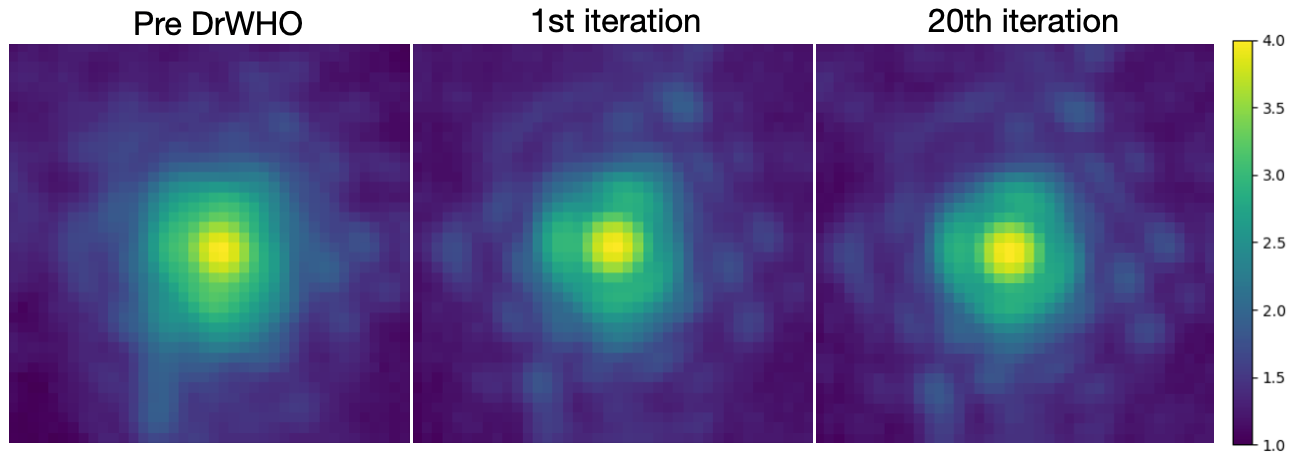
\includegraphics[width=0.47\textwidth]{fig/Dec7nightresult.png}
\caption{Evolution of the on-sky PSF before running the algorithm, after the first iteration, and the after last iteration. Each image is 0.25~arcsec (40x40 pixels) across, acquired at $\lambda = $ 750~nm, 30 sec exposure time (computed by co-addition of 15,000 frames acquired at 500~Hz).}
\label{fig:SkyResult}
\end{figure}




\begin{figure}[t]
\centering
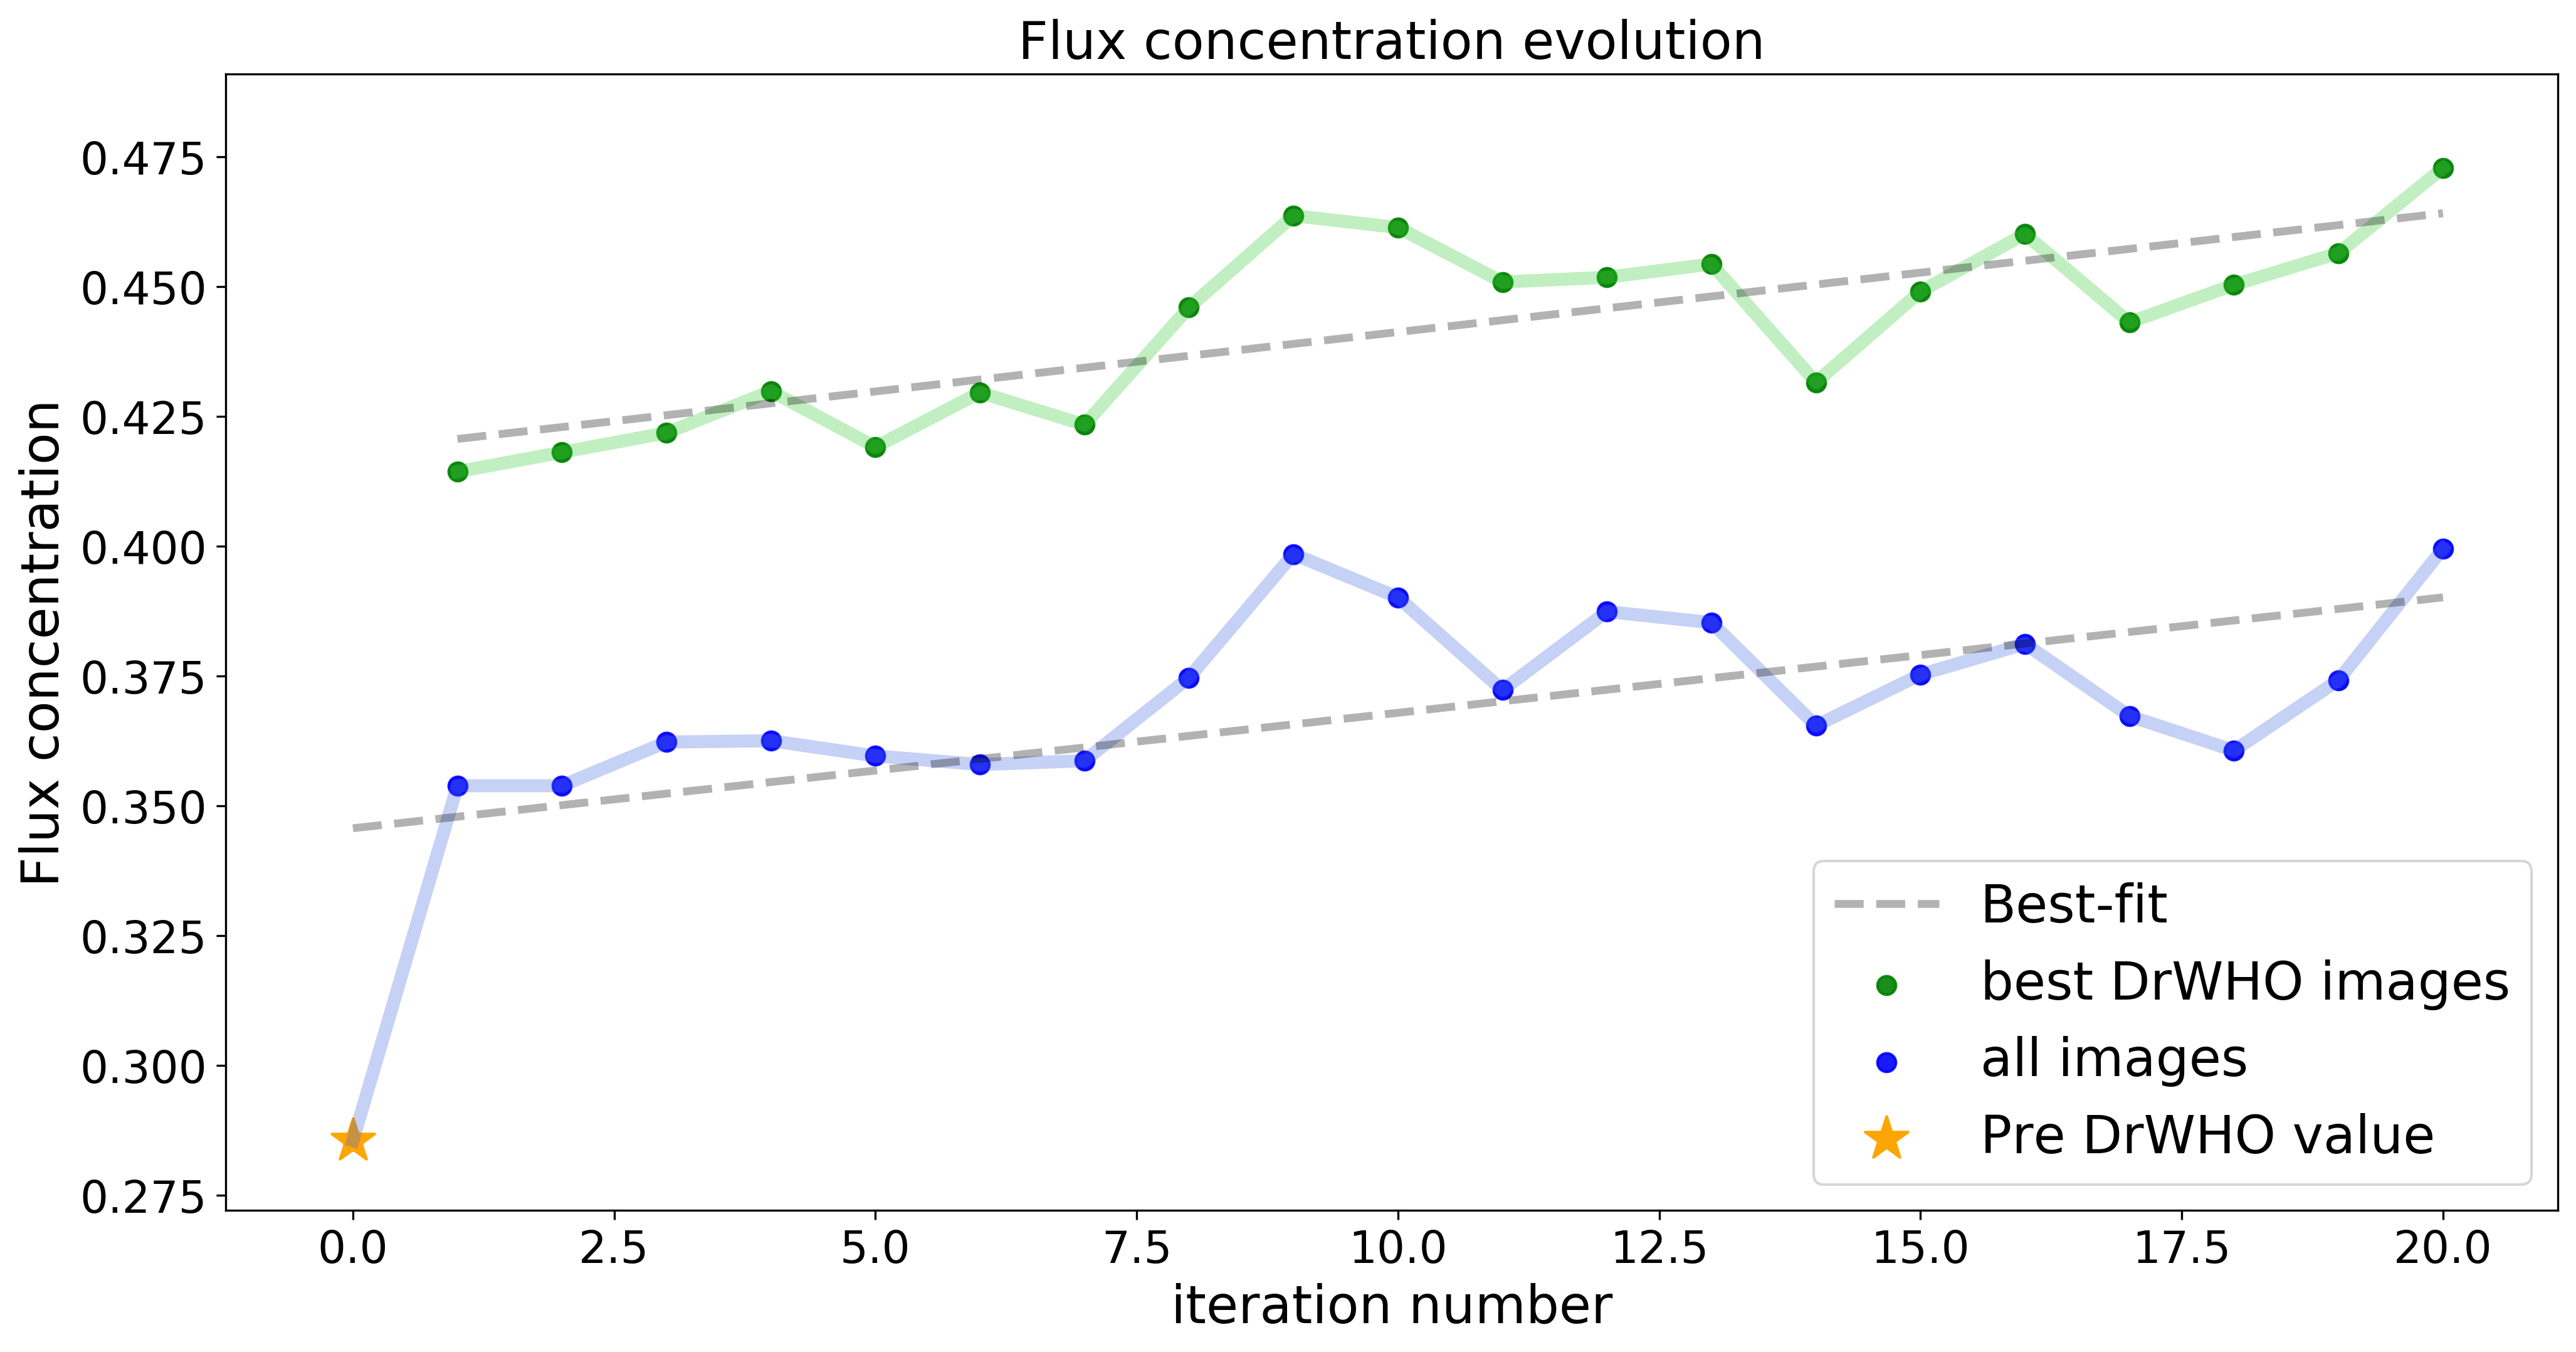
\includegraphics[width=.5\textwidth]{fig/NNevolution.png}
\caption{Evolution of the FC over 20 iterations of DrWHO, corresponding to a period of 10 minutes, including the nFC of the PSF preceding the run. 
%The nFC was calculated for a window of 40x40 pixels, normalised by the FC of an ideal PSF as shown in figure \ref{fig:perfect_psf}. 
The blue curve corresponds to the evolution of the nFC of all the PSF averaged over the DrWHO iteration, while the green one corresponds to the evolution of the nFC of the 10\% PSF chosen by DrWHO. The best linear fit is presented. }
\label{fig:NNevolion}
\bigbreak
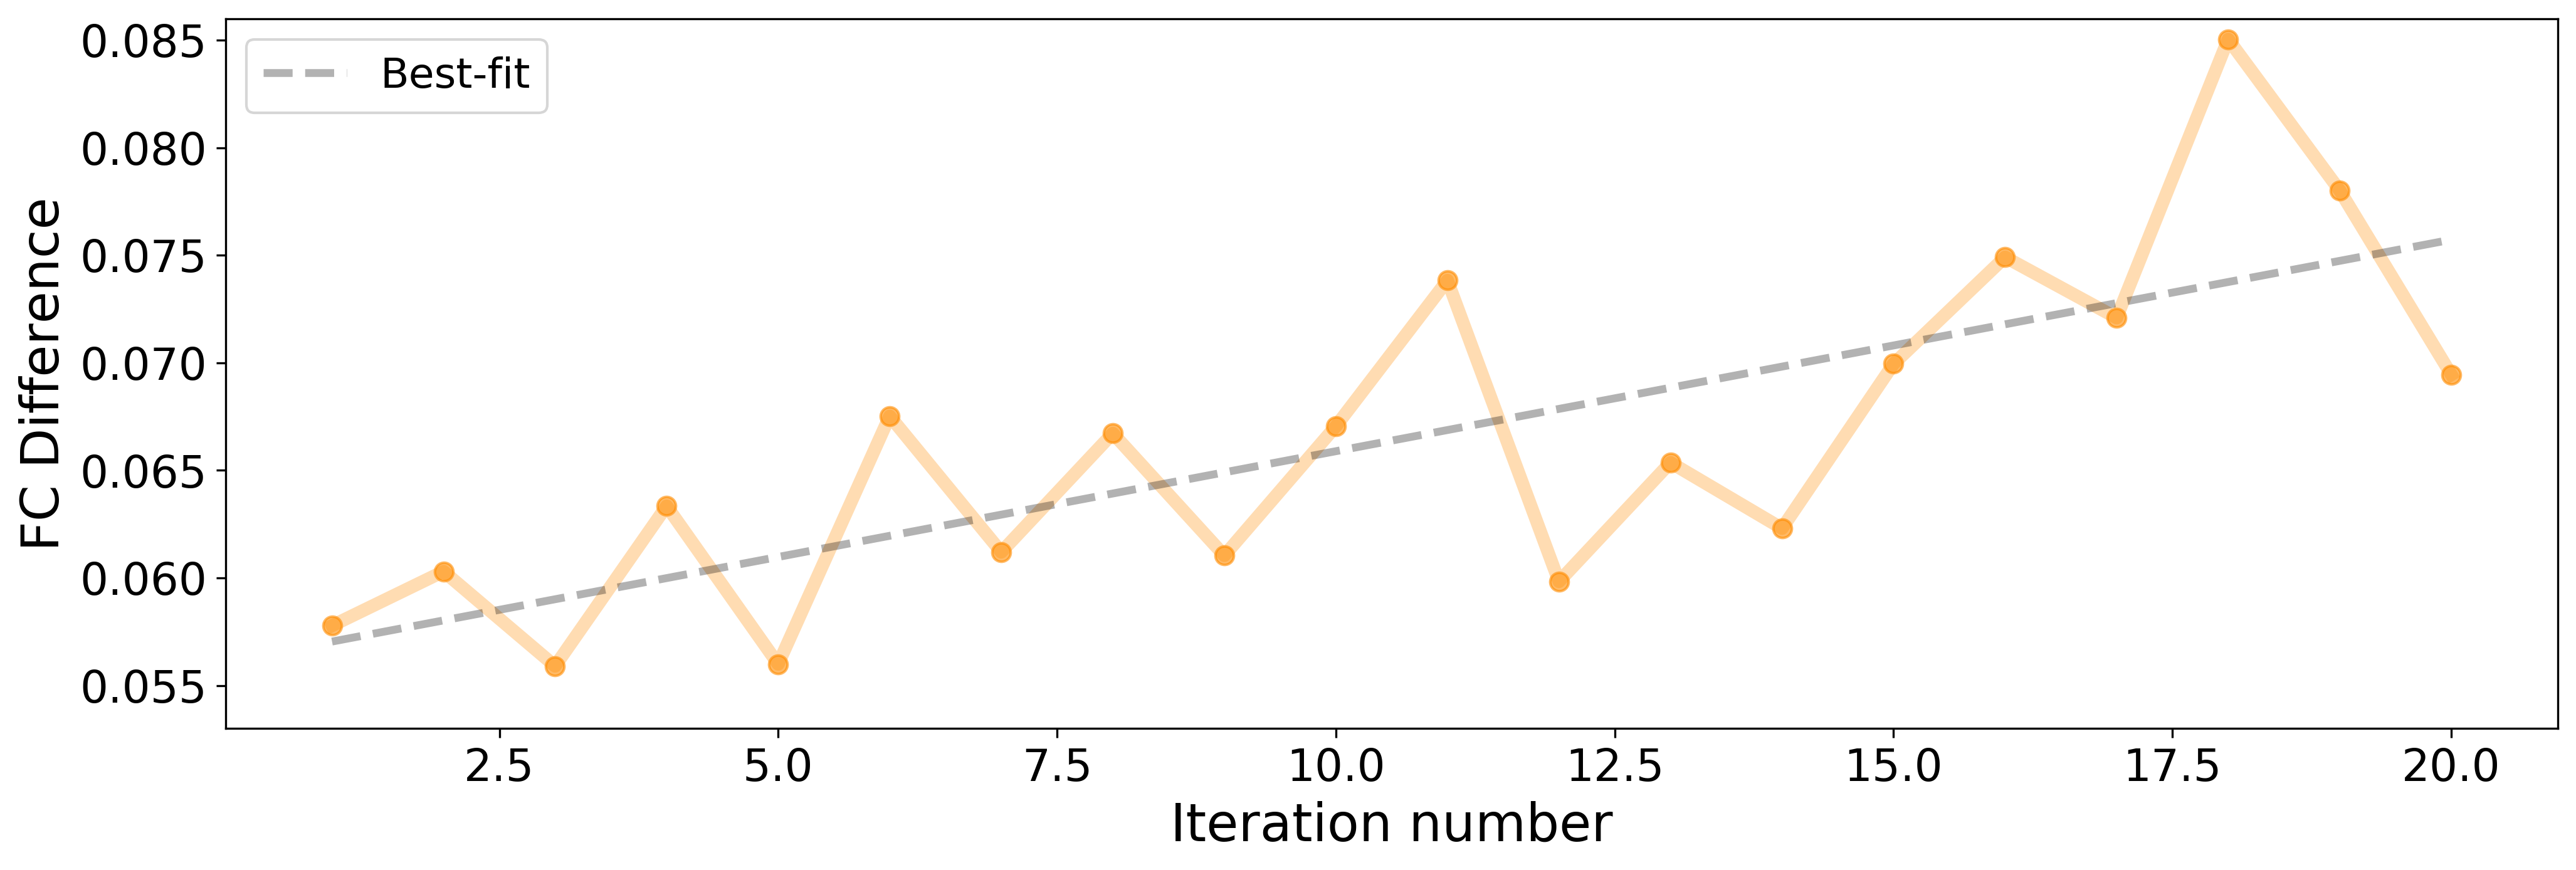
\includegraphics[width=.5\textwidth]{fig/difference.png}
\caption{Difference between the nFC of the mean of the best 10\% images, and the nFC of the mean of all the PSFs, over 20 iterations of DrWHO. We calculated the best linear fit to better understand the increase of the difference.}\label{fig:difference}
\end{figure}


%According to Figure \ref{fig:NN4040}, the PSF flux is initially spread over 15.5 pixels, and after the 20 iterations of DrWHO, there is a gain of 1 pixel and the flux is spread over 14.6 pixels. \\

%\subsection{Telemetry}
%The first step taken was to look at the telemetry of previous nights and on one iteration of the DrWHO loop, do some kind of reverse engineering to figure out the success level of the iteration on the data cube. We look at the reference output by DrWHO, we look at the WFS images that are close to it, and then take the corresponding PSF and we prove it's of better quality than the average of all the PSFs. 

\subsection{Evolution of the WFS reference}

Figure \ref{fig:reference_diff} compares the WFS reference prior DrWHO, \textit{Ref0}, which is the WFS mask showing which pixels are active (i.e. respond to DM pokes) in the WFS image, and the average of the last 3 WFS references applied by DrWHO, during the on-sky 10-minute run. The averaging minimises the noise contribution. 

In order to better understand the action on the reference of the PyWFS, we measured the difference between these two references, the \textit{Ref0} and the average of the three last DrWHO references. The image is shown in Figure \ref{fig:reference_diff}. This difference was then converted to wavefront mode coefficients by multiplication by the control matrix. Modal coefficients are shown in Figure \ref{fig:modes_proj} where the first three modes are tip, tilt, and defocus and the following modes correspond to orthogonal modes, optimized for SCExAO's AO control law.


% Table \ref{tab:mode_contribution} presents the contribution of blocks of modes (without tip-tilt):
The total contribution of all modes is of 116.3~nm RMS. However, as seen on Figure \ref{fig:modes_proj}, the high order modes, corresponding to the higher spatial frequencies, seem to be noise more than actual correction, which will be further explored thereafter. 

When calculating the total contribution of the modes by removing the modes beyond 900, we compute a correction of 70~nm RMS.

\begin{figure}[t]
\centering
%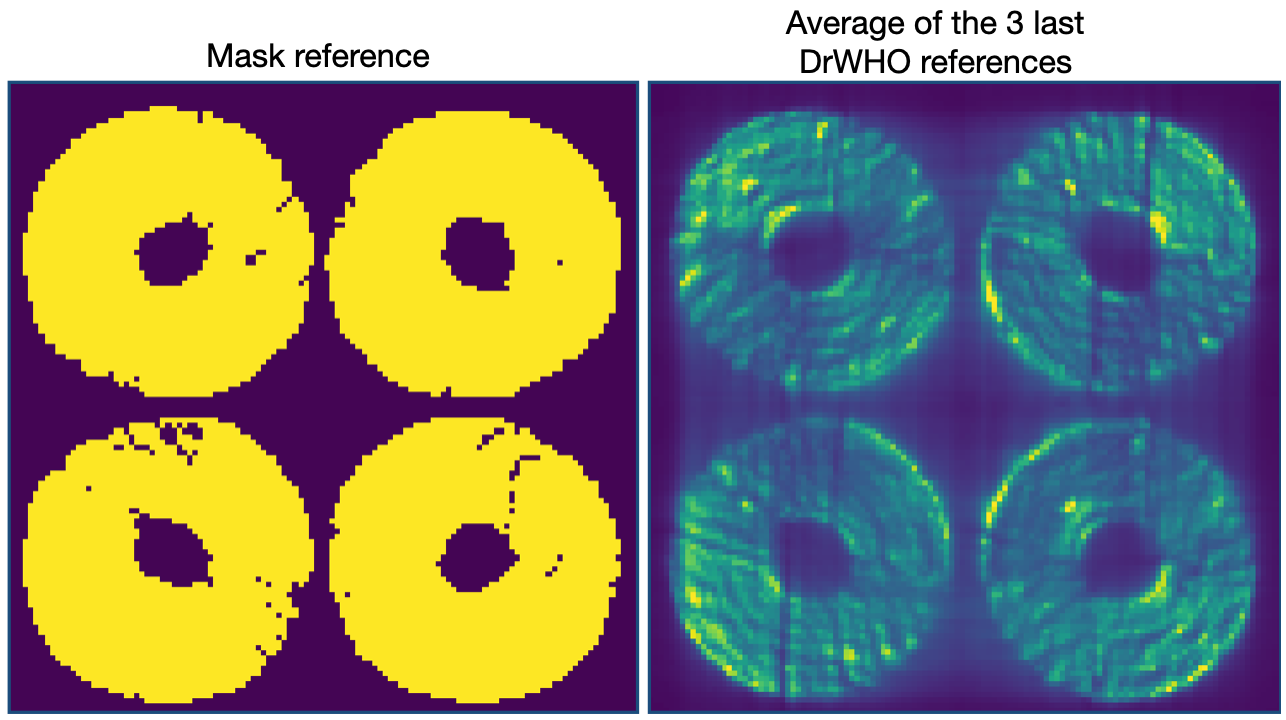
\includegraphics[width=.45\textwidth]{fig/WFSref_comp.png}
%\caption{}
%\label{fig:WFSref_comp}
%\bigbreak
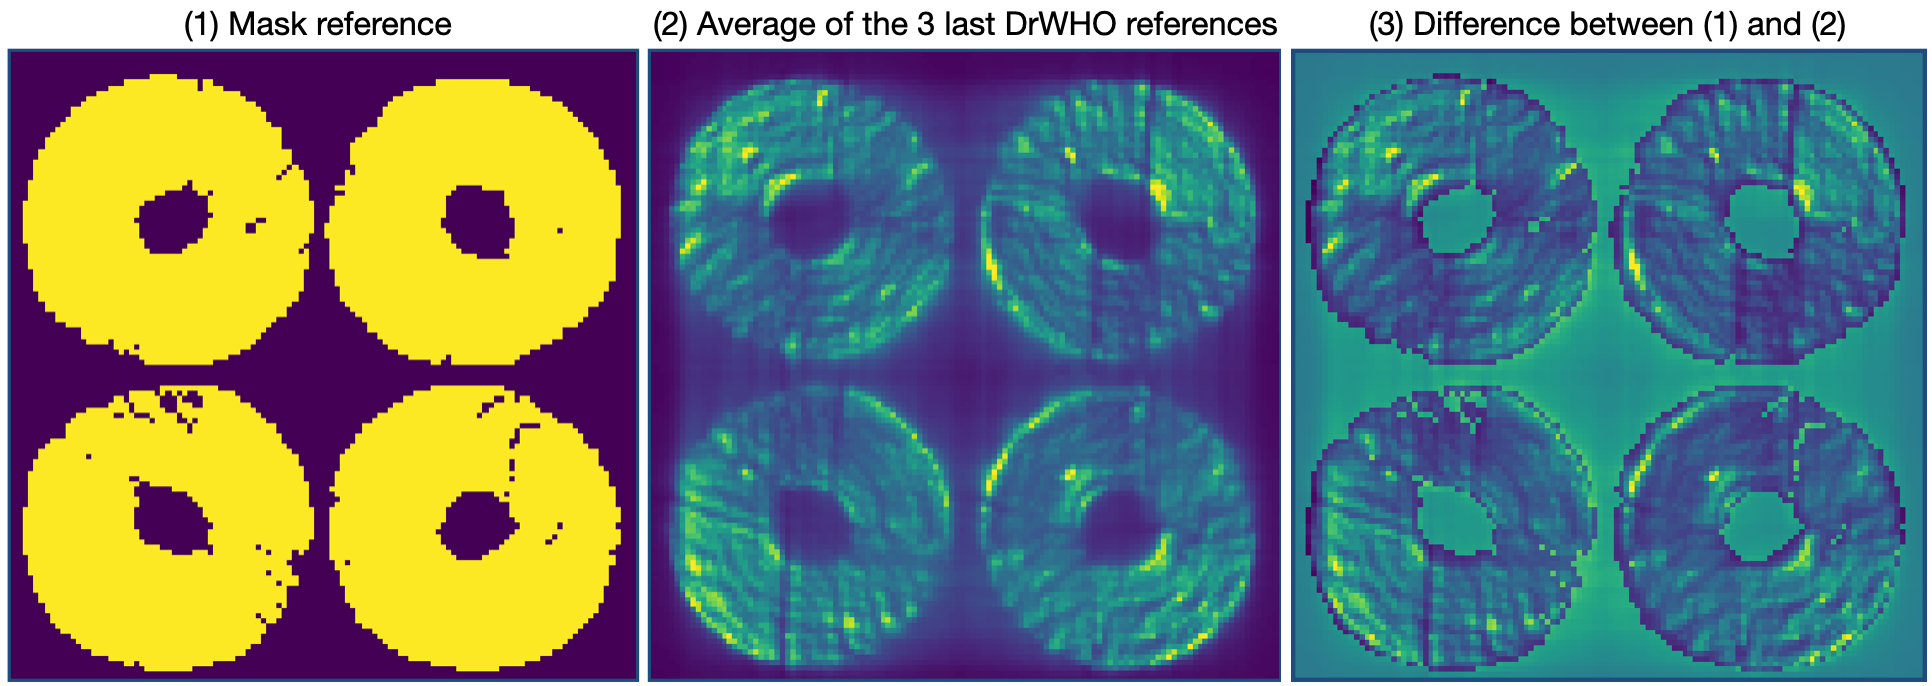
\includegraphics[width=.48\textwidth]{fig/reference_diff.png}
\caption{Left: images of the PyWFS reference before the first iteration, referred to as \textit{Ref0}, set equal to the WFS mask. Middle: average of the last 3 iterations of DrWHO WFS references. The contrast scale for this image has been modified for better visualisation. Right: difference between the two images in the left and in the middle.}
\label{fig:reference_diff}
\end{figure}


Figure \ref{fig:10_modes} shows the first 20 wavefront mode values, excluding tip-tilt. Focus is the dominant contribution to the aberrations, with an amplitude of nearly 14~nm. We furthermore note that the higher modes from approximately the mode 900 to 1217, corresponding to higher frequencies, seem to have a considerable contribution in the overall correction. One would wonder whether those higher order contributions are just random noise, or meaningful behavior. We plotted the evolution of one example of a high mode (arbitrarily chosen for this paper to be the mode 1120), in the bottom of Figure \ref{fig:10_modes}. After the first iteration, the algorithm converges very rapidly towards a value of about -9~nm, with a standard deviation of approximately 2~nm RMS, which probably corresponds to a noise contribution. This observation is valid for the entirety of the high order modes. Table \ref{tab:mode_contribution} presents the contribution of the modes in nm RMS, in the following cases: in considering all the modes except tip-tilt (from 2 to 1217) ; then in removing the higher order modes (from 2 to 900 only) to show what the contribution would be without the higher spatial frequencies ; then the low order modes (from 2 to 20), and finally the focus contribution, which is  13.9~nm. 


\begin{figure}[t]
    \centering
    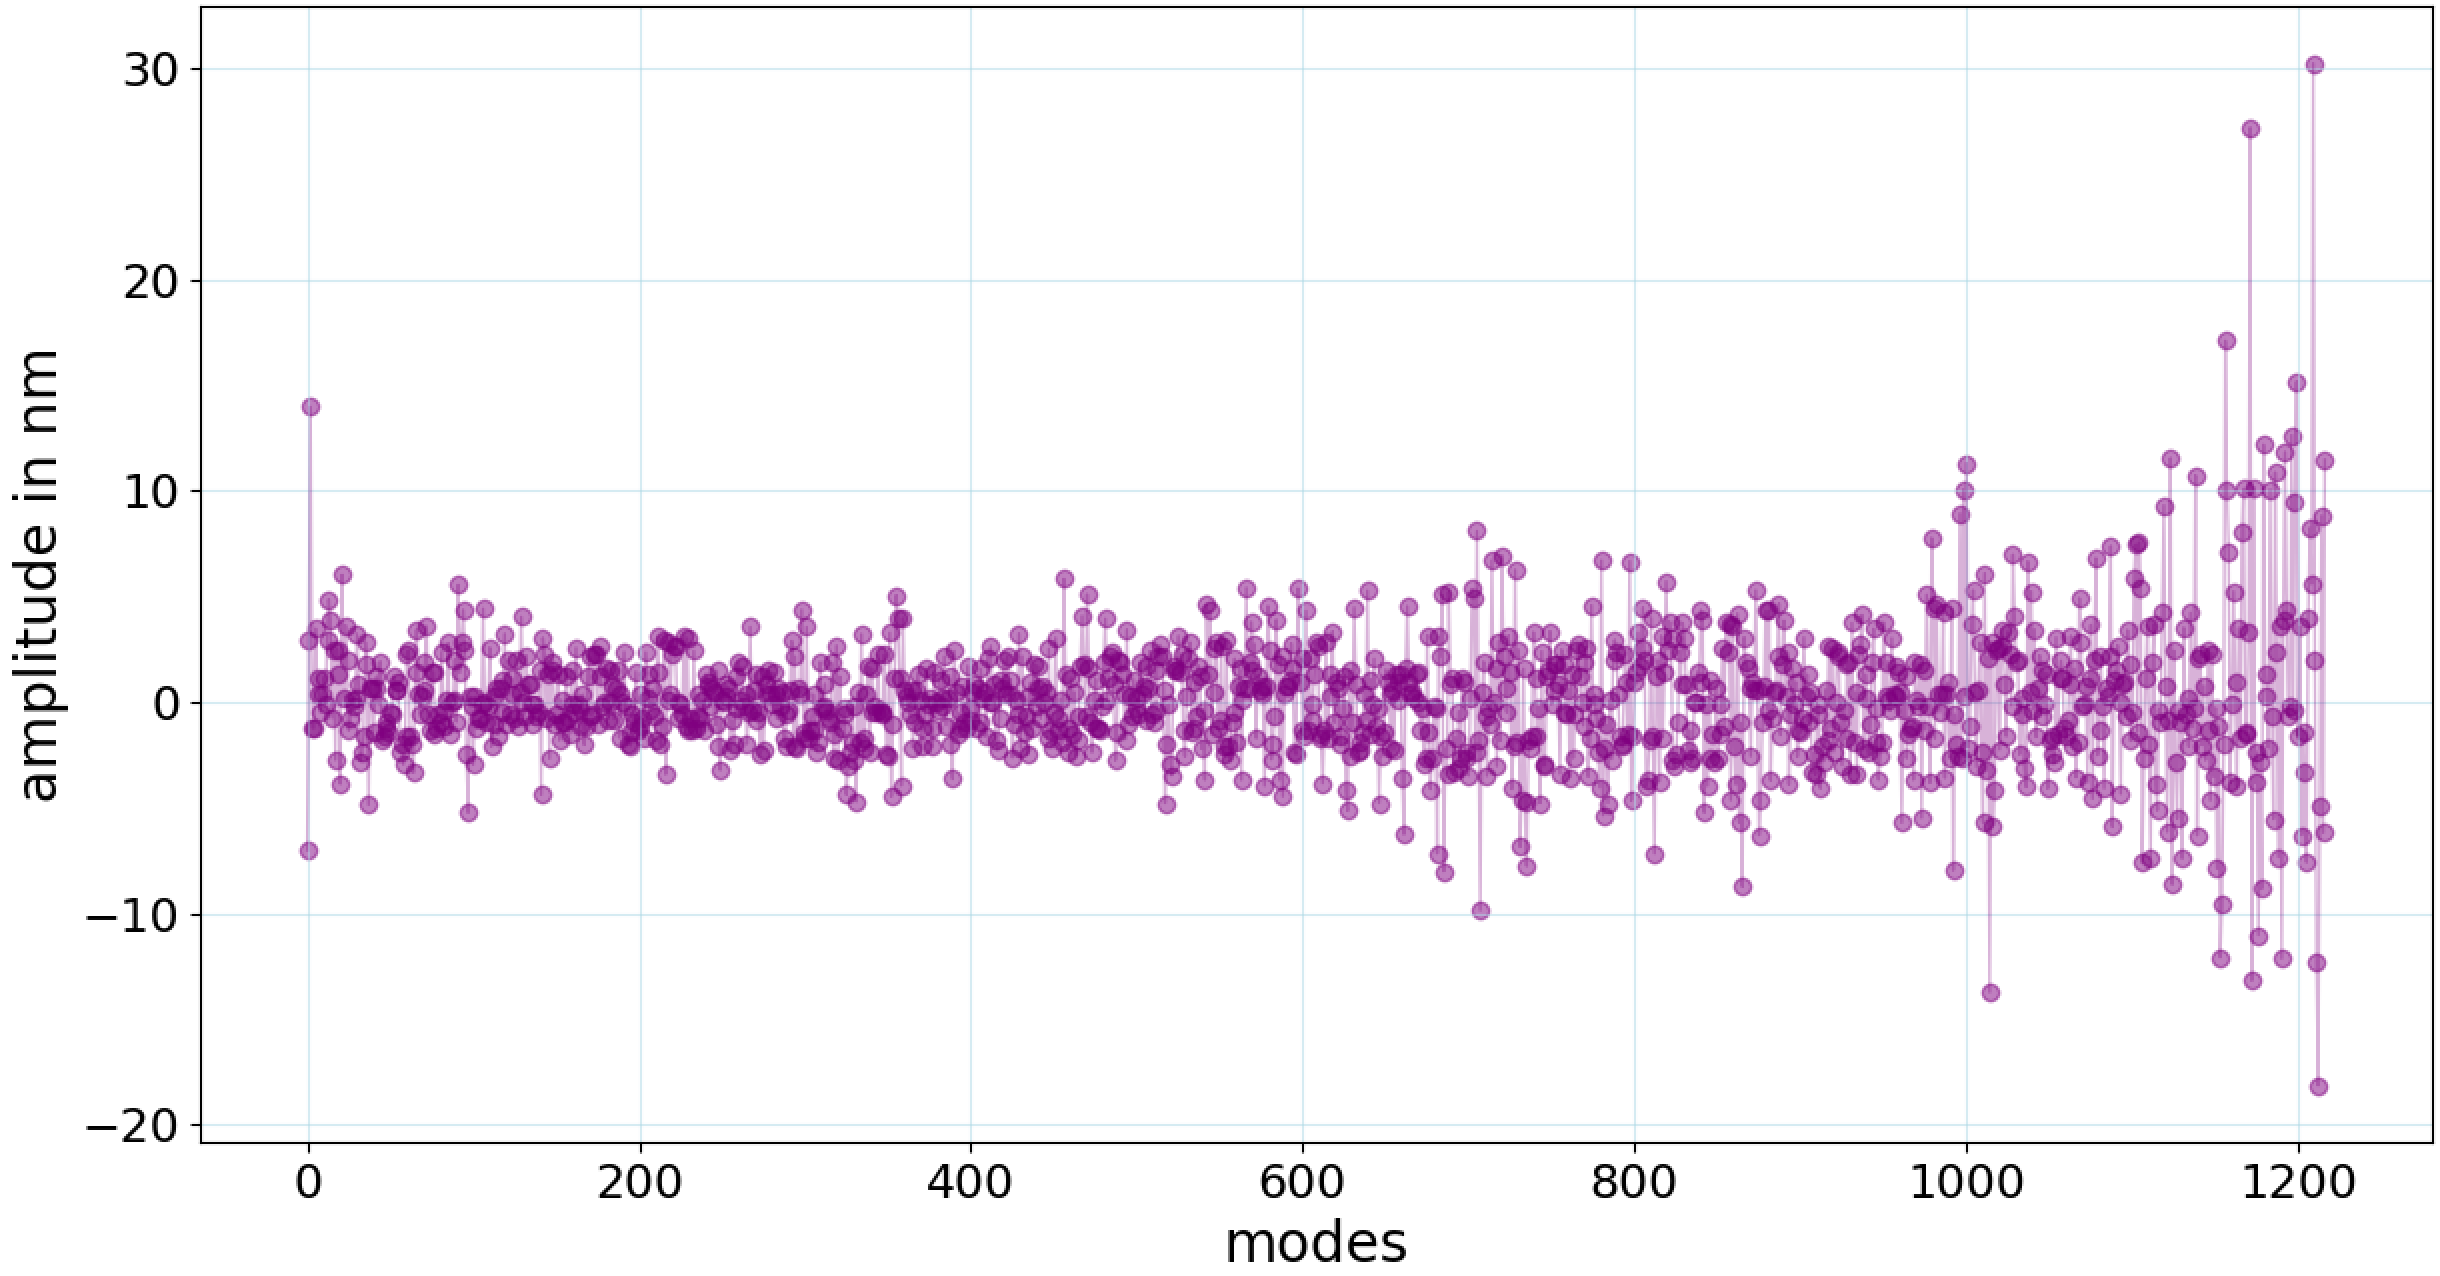
\includegraphics[width=.43\textwidth]{fig/modes_proj.png}
    %\caption{(a)}
    \caption{Modal decomposition of DrWHO correction, computed from the difference between the pre-DrWHO WFS reference and the average of the WFS references for the last 3 DrWHO iterations.}
    \label{fig:modes_proj}
    \bigbreak
    %
    %
    %
    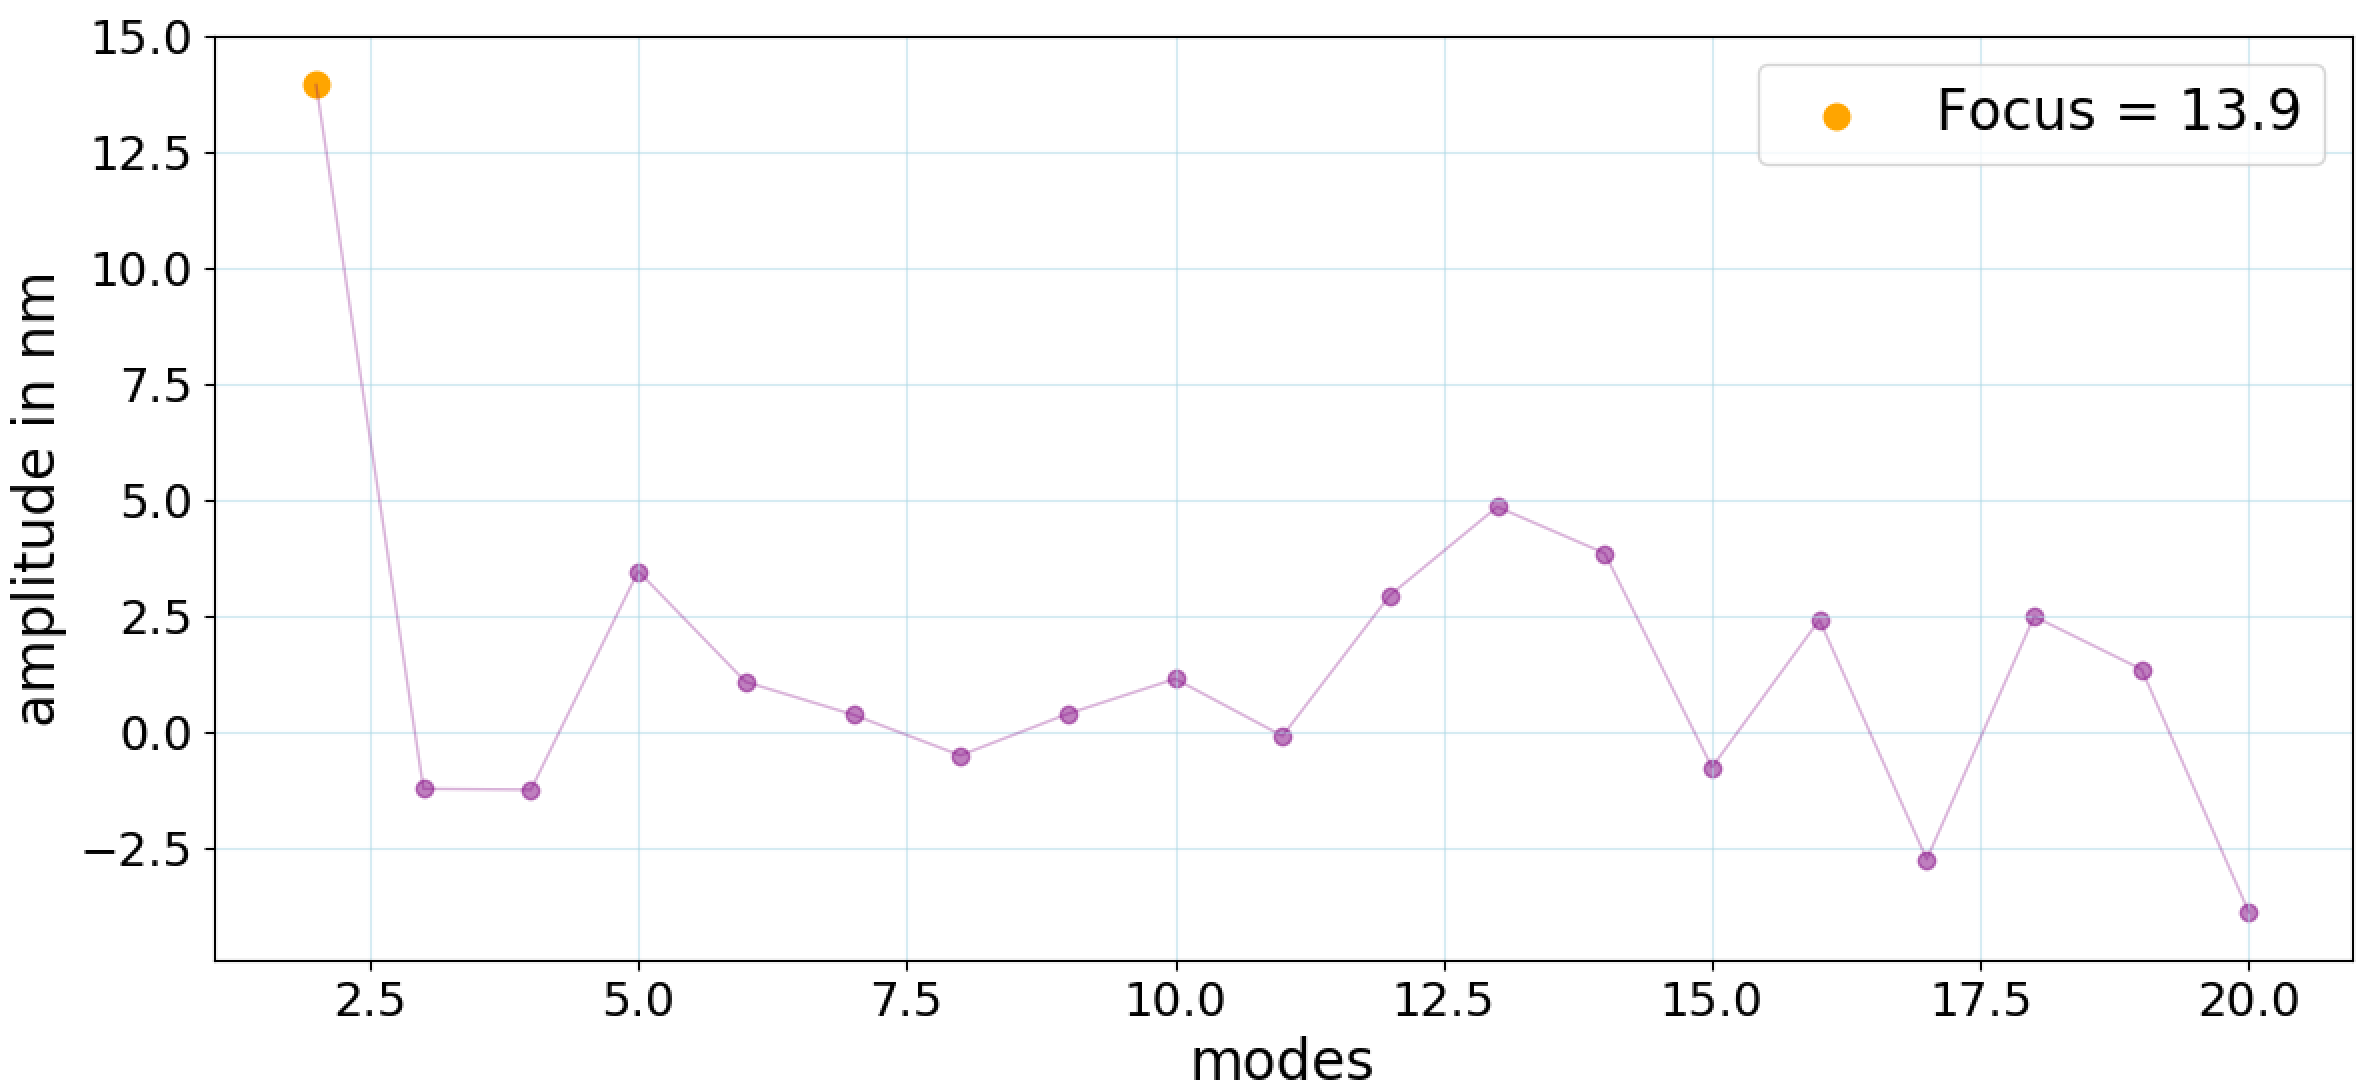
\includegraphics[width=.4\textwidth]{fig/10_modes.png}\\
    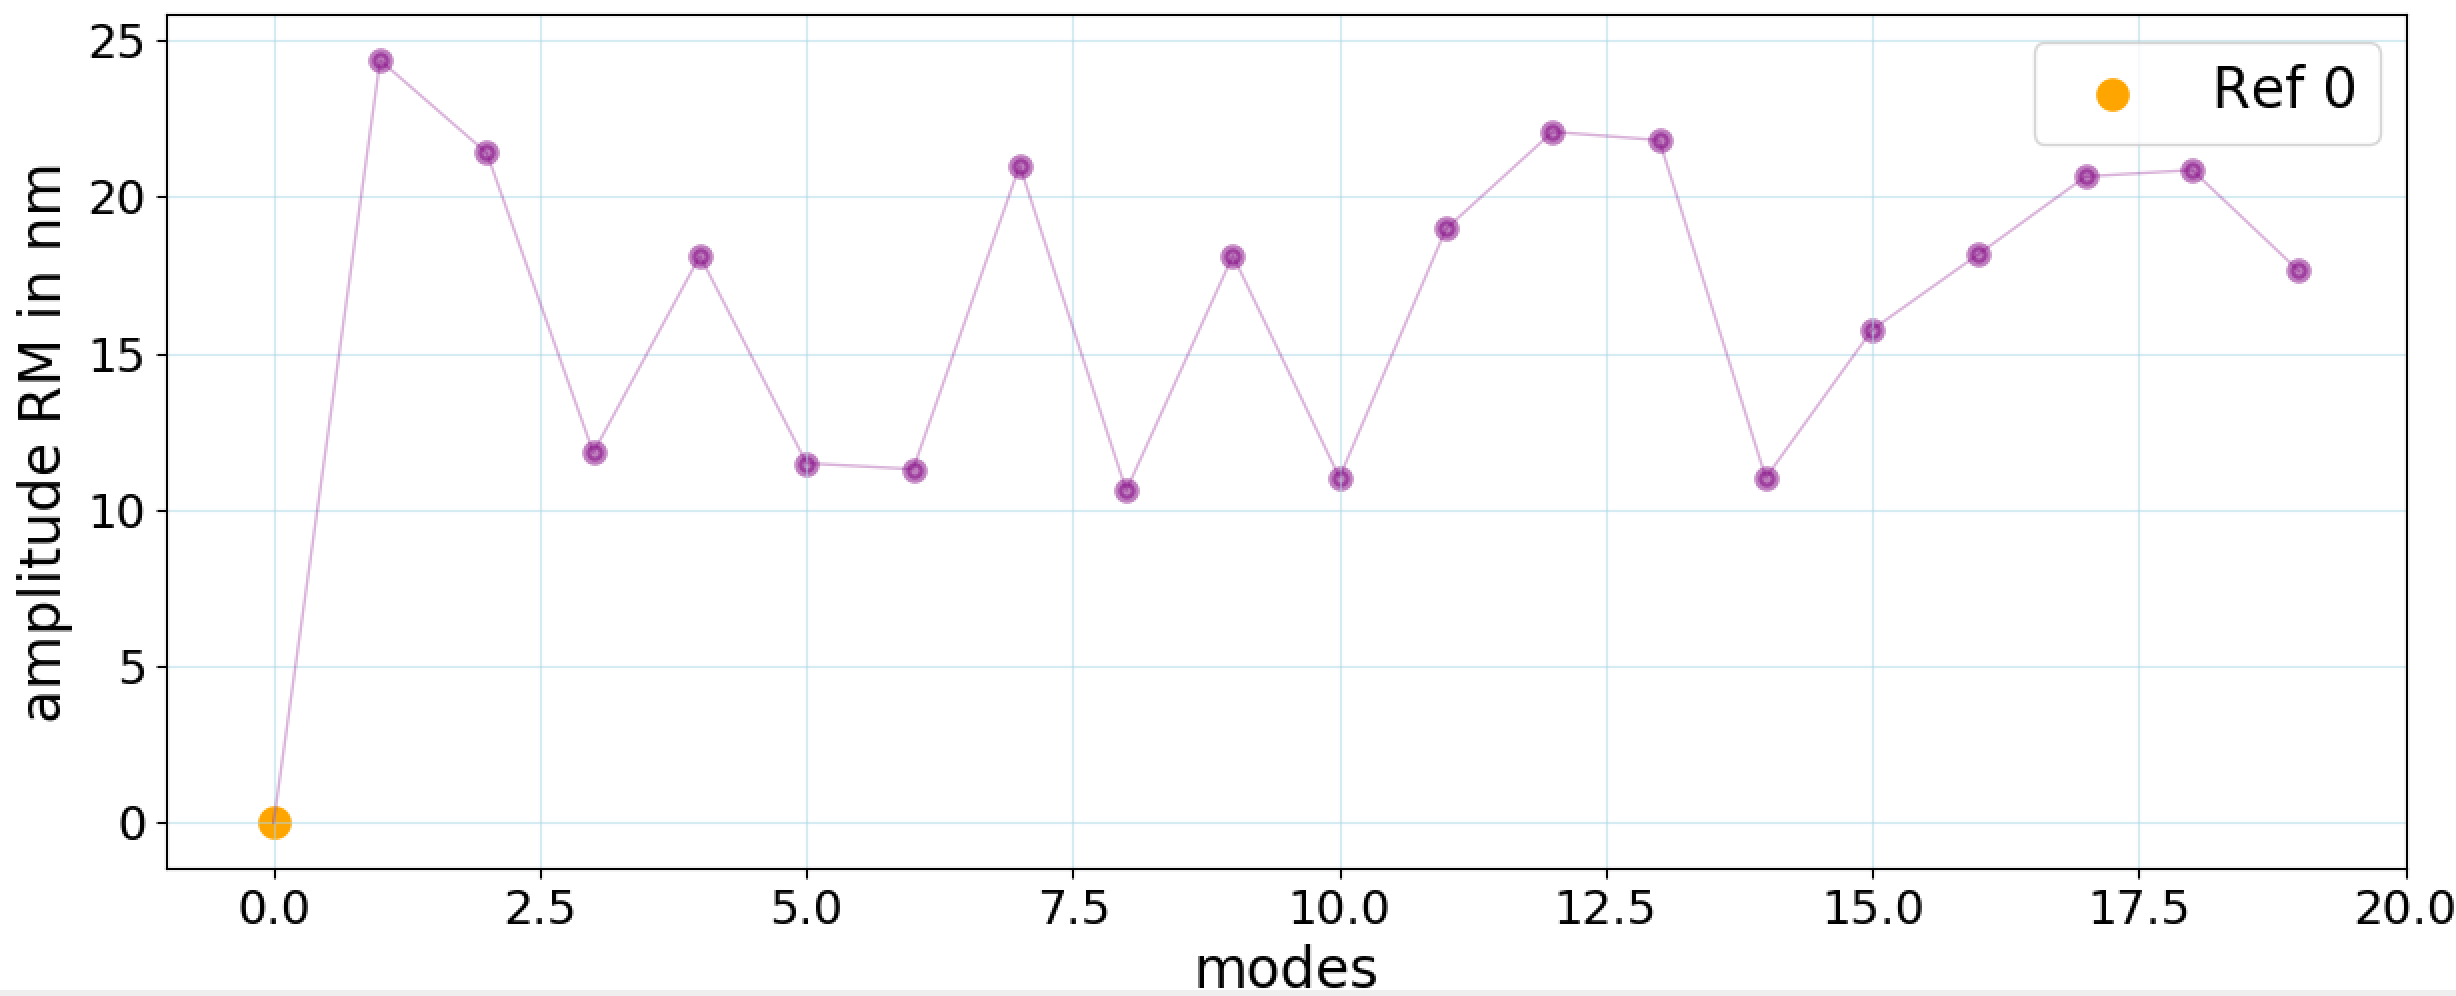
\includegraphics[width=.4\textwidth]{fig/defoc_evolution.png}\\
    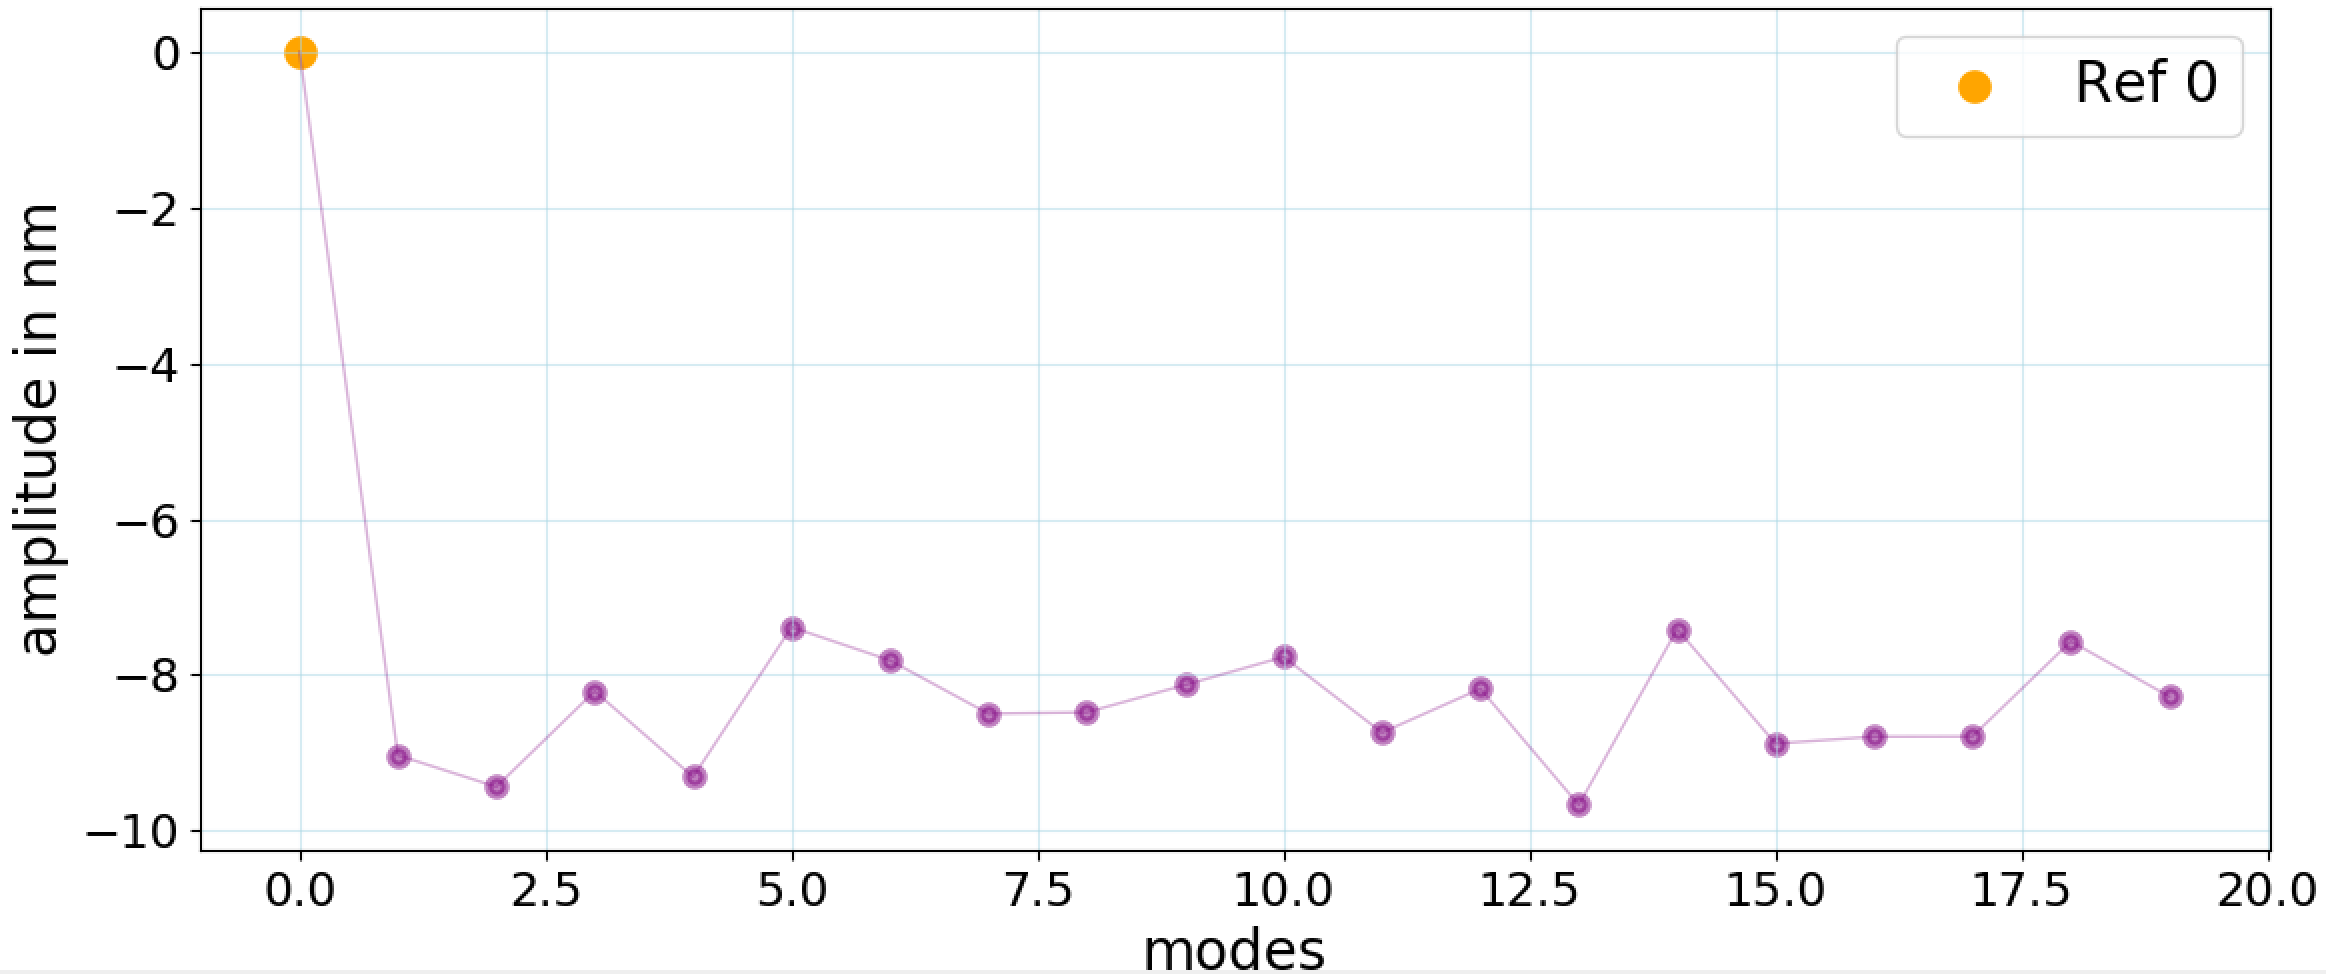
\includegraphics[width=.4\textwidth]{fig/mode1120.png}
    %\caption{(b)}
    \caption{Top: modal decomposition of DrWHO correction for the first 20 modes, excluding tip-tilt. Focus is the major contributor with an amplitude of 13.9~nm RMS. %}
    %\caption{
    Middle: evolution of the focus WFS reference correction during the DrWHO run. %}
    %\caption{%
    Bottom: evolution of high order mode 1120 WFS reference correction during the DrWHO run. }
    \label{fig:10_modes}
    %\caption{(c)}
    %\label{fig:defoc}
    %\caption{(d)}
    %\label{fig:mode1120}
\end{figure}

\begin{table}[ht]
\begin{tabular}{c|l|l|l|l}
\textbf{Modes}                                                            & 2 to 1217 & 2 to 900 & 2 to 20 & \multicolumn{1}{c}{Focus} \\ \hline
\textbf{\begin{tabular}[c]{@{}c@{}}Contribution \\ (nm RMS)\end{tabular}} & 116.3     & 70.3     & 17.2    & 13.9   
\end{tabular}
\caption{Contribution of the modes of the difference of Figure \ref{fig:difference} in nm RMS}
\label{tab:mode_contribution}
\end{table}



\section{Discussion}\label{sec:Discussion}
Below are some noticeable characteristics of the DrWHO algorithm that have been demonstrated: 
\begin{enumerate}
    \item It is robust: the algorithm slowly but surely converges towards a better compensation of static and slow aberrations. As it is based on lucky imaging, it relies on some realisations of residual atmospheric turbulence to reduce wavefront aberrations. DrWHO contributes to getting closer to an absolute sensor, driving the WFS reference to optimize PSF in the focal plane.
    \item It does not rely on any model, and does not rely on using the DM for probing, making it compatible with other wavefront control techniques: DrWHO's approach is different from active cancellation speckle, because it simply does a statistical selection.
    \item It does not require modification of the AO loop control scheme other than WFS reference updates.
    \item It does not make any linear assumption, so it is not concerned with non-linearities of the system, such as WFS non-linearity.
    \item It is flexible in the parameters, whether it is the score (Strehl, contrast, intensity, etc.), or the selection fraction and the time of the iteration, making it adaptable to different weather conditions and AO systems with different characteristics and scientific goals.
    \item However, DrWHO needs a fast focal plane camera as close as possible from the science camera, to more accurately compensate the NCPAs and low aberrations. 
    %\item \nour{Need to add a point about higher orders and their consistency throughout the iterations}
    
\end{enumerate}

On-sky tests were run on a bright star, but the algorithm efficiency must be improved to run on fainter targets, and be able to optimise deep contrast for HCI. Indeed, there are two main points to be emphasized regarding future improvements of the algorithm, which will be presented in future papers: 
\begin{enumerate}
    \item It is applicable to HCI with coronagraphic images, where it would be exactly the same thing as what is presented here, but with adapting the quality criteria of the selection. In this case, instead of selecting PSFs with the maximum FC, image contrast would be optimized.
    \item There are numerous ways to improve the algorithm efficiency and convergence speed. For example, a possible extension is to parallelize DrWHO in terms of spatial frequencies. If there is a good understanding of the relationship between the input wavefront and the focal plane, as for example a Fourier relationship, DrWHO can optimize separate spatial frequencies independently. 

\end{enumerate}


\section{Conclusion}

The DrWHO algorithm has been tested in numerical simulations, and then deployed and validated on-sky with the SCExAO instrument at the Subaru Telescope. Results presented in this paper demonstrate its ability to measure and compensate for NCPAs, considered to be a limiting factor in the detection and characterisation of exoplanets in high-contrast imaging observations. To quantify the quality of the PSF, we used the Strehl ratio for the simulations, and the \textit{Flux Concentration} - that we defined here - for the SCExAO run. On sky, the PSFs used to run the algorithm were from the VAMPIRES instrument, in the visible. When DrWHO was running, the PSF significantly improved (12\% relative improvement in flux concentration) over 20 iterations of 30 seconds, for a total of 10 minutes. The best PSF have a sharper increase over the run of the algorithm, reaching 48\% of the simulated ideal PSF flux concentration.

This shows that DrWHO is able to improve the wavefront quality arriving on the science camera, and partially correct for the static and quasi-static NCPAs, over a relatively short period of time of a few seconds. We show that the algorithm converges rapidly, with about half of the correction achieved by the first iteration. This has been observed in simulation and on-sky.

The characteristics of DrWHO are enumerated in section \ref{sec:Discussion}. The main strong points are the robustness of the algorithm, its independence from any model, making it compatible with other wavefront control methods, and that it does not rely on any linear assumption, thus particularly fit for a PyWFS.
In fact, some other techniques for compensating NCPAs mentioned in section \ref{sec:intro} usually work independently from the WFS. They do their own correction based on a model, for example applying probes on a DM channel that is parallel to the AO loop DM channel. DrWHO combines focal plane wavefront sensing and the WFS. \\
Furthermore, there is a natural extension of this technique in high contrast imaging to be more efficient by parallelizing in terms of spatial frequencies, which would allow to correct speckles individually and go would allow to observe fainter targets. 

Operating DrWHO requires the access to two data streams: the WFS measurements, and a short exposure focal plane camera, which ideally would be the closest possible to the science camera to correct the NCPAs in the most accurate way possible. It is befitting for observations. \\

This paper is the first proof of concept of the algorithm, and presents some first results of its PSF quality and stability enhancement. DrWHO shows a wide potential of improvement, which will be presented in future work.




\begin{acknowledgements}
The development of SCExAO was supported by the Japan Society for the Promotion of Science (Grant-in-Aid for Research \#23340051, \#26220704, \#23103002, \#19H00703 \& \#19H00695), the Astrobiology Center of the National Institutes of Natural Sciences, Japan, the Mt Cuba Foundation and the director's contingency fund at Subaru Telescope. The authors wish to recognize and acknowledge the very significant cultural role and reverence that the summit of Maunakea has always had within the Hawaiian community. We are most fortunate to have the opportunity to conduct observations from this mountain. NS acknowledges support from the PSL Iris-OCAV project. NS and VD acknowledge support from NASA funding (Grant \#80NSSC19K0336). 
\end{acknowledgements}


\bibliographystyle{aa}
\bibliography{main}


\end{document}